\label{sec:techniques}

This chapter reviews the computational techniques used to solve the governing
equations presented in the previous chapter for the geometries of interest.

\section{Numerical Discretization}
\label{sec:discretization}

The target geometries are channels and flat plates with coordinates as depicted
in \autoref{fig:geometry}.  The former geometry requires nearly a proper subset
of the capabilities necessary to solve the latter and is used for validation
purposes in \autoref{sec:software}.  The flat plate geometry is the subject
of Chapters~\ref{sec:bldata} and~\ref{sec:relam}.
The streamwise and spanwise directions are formally infinite which is emulated
using periodicity in these directions in conjunction with a sufficiently large
domain.

\begin{figure}
\centering
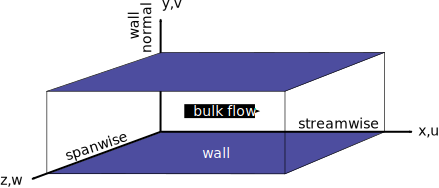
\includegraphics[width=0.495\textwidth]{ChannelSchematic}
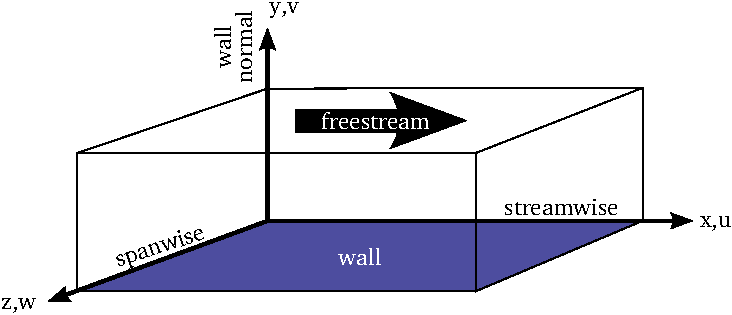
\includegraphics[width=0.495\textwidth]{FlatPlateSchematic}
\\
\caption[The channel and flat plate geometries]{%
  The channel (left) and flat plate (right) geometries. \label{fig:geometry}
}
\end{figure}

A mixed Fourier--Galerkin/B-spline collocation spatial
discretization is combined with a low-storage, semi-implicit third-order
Runge--Kutta scheme.  The spatial discretization yields excellent spectral
resolution~\citep{Kwok2001}, has long been proven for supersonic,
spatially homogenized boundary layer simulations~\citep{Guarini2000Direct}, and
provides a natural, scalable parallel domain decomposition on high-performance computing
environments.  The temporal discretization, used repeatedly at large
scale~\citep[e.g.][]{Hoyas2006Scaling} since its
introduction~\citep{spalart_lowstoragerk}, mitigates the potentially severe
acoustic and diffusive stability limits present in our problems of interest.
Nondimensional density $\rho$, momentum $m=\rho{}u$, and total energy
$e=\rho{}E$ were used as state variables.

%While many of the choices documented below have practical ramifications for
%the proposed simulation campaign and represent a large part of the work
%completed to date, the numerics are not genuinely new.  Accordingly, \emph{the
%remainder of this subsection may be skipped without loss of continuity.}

\subsection{Fourier/B-Spline Spatial Discretization}
\label{sec:spatialdiscretization}

Mimicking the governing equations in \autoref{sec:goveqn}, consider the abstract
continuous system
\begin{align}
  \frac{\partial\!u}{\partial\!t} &= \mathscr{L}u + \mathscr{N}\!\left(u\right)
\end{align}
on the spatial domain $\left[-\frac{L_x}{2},\frac{L_x}{2}\right] \times{}
[0,L_y] \times{} \left[-\frac{L_z}{2},\frac{L_z}{2}\right]$.  The operators
$\mathscr{L}$ and $\mathscr{N}$ are linear and nonlinear, respectively.
%For
%brevity, this section suppresses any time dependence in the operators.
To discretize this system, introduce its finite dimensional analog
\begin{align}
  \frac{\partial\!u^h}{\partial\!t}
  &=
  \mathscr{L}u^h + \mathscr{N}\!\left(u^h\right) + R^h
  \label{eq:discrete_system_with_residual}
\end{align}
where the continuous field $u = u\!\left(x,y,z,t\right)$ has been replaced by the discrete
field $u^h = u^h\!\left(x,y,z,t\right)$ with $N_x\times{}N_y\times{}N_z$ degrees of
freedom, and $R^h$ is the discretization error.
Fourier expansions are selected for the periodic $x$ and $z$ directions while a
B-spline expansion is adopted for the aperiodic $y$ direction.  That is,
\begin{align}
u^h(x,y,z,t)
&=
  \sum_{l=0}^{N_y - 1}
  \sum_{m=-\frac{N_x}{2}}^{\frac{N_x}{2}-1}
  \sum_{n=-\frac{N_z}{2}}^{\frac{N_z}{2}-1}
  \hat{u}_{l m n}(t)
  B_l\!\left(y\right)
  e^{\ii\frac{2\pi{}m}{L_x}x}
  e^{\ii\frac{2\pi{}n}{L_z}z}
  \notag\\
&=
  \sum_{l}\sum_{m}\sum_{n}
  \hat{u}_{l m n}(t)B_l\!\left(y\right)e^{\ii k_m x}e^{\ii k_n z}
  \label{eq:u_h_expansion}
\end{align}
where $k_m = 2\pi{}m/L_x$, $k_n = 2\pi{}n/L_z$, and $B_l\!\left(y\right)$ are a
B-spline basis for some order and knot selection.

Applying the method of weighted residuals, a mixed Galerkin/collocation
approach (often called a ``pseudospectral'' technique) is chosen that employs
the $L_{2}$ inner product and test ``functions'' like $\delta(y-y_{l'}) e^{\ii
k_{m'} x}e^{\ii k_{n'} z}$ where $l'$, $m'$, and $n'$ range over the same
values as $l$, $m$, and $n$, respectively.  The fixed collocation points
$y_{l'}$ depend on the B-spline basis details.  Three orthogonality
results are
\begin{subequations}
\begin{align}
   \int_0^{L_y} \varphi(y) \, \delta(y-y_{l'}) \,d\!y
&= \varphi(y_{l'})
\\
   \int_{-\frac{L_x}{2}}^{\frac{L_x}{2}} e^{\ii k_m x} e^{-\ii k_{m'} x} \,d\!x
&= L_x \delta_{m m'}
\\
   \int_{-\frac{L_z}{2}}^{\frac{L_z}{2}} e^{\ii k_n z} e^{-\ii k_{n'} z} \,d\!z
&= L_z \delta_{n n'}
\end{align}
\end{subequations}
where the inner product's conjugate operation is accounted for by introducing a
negative sign into the latter two exponentials.  The weighted residual is
forced to be zero in the sense that
\begin{align}
  \int_0^{L_y}
  \int_{-\frac{L_x}{2}}^{\frac{L_x}{2}}
  \int_{-\frac{L_z}{2}}^{\frac{L_z}{2}}
  R^h\!\left(x,y,z\right) \delta(y-y_{l'}) e^{-\ii k_{m'} x}e^{-\ii k_{n'} z}
  \,d\!z \,d\!x \,d\!y
  &=
  0
  \label{eq:R_h_weighted_residual_zero}
\end{align}
holds for all $l'$, $m'$, and $n'$.  Inserting \eqref{eq:u_h_expansion} into
\eqref{eq:discrete_system_with_residual}, testing with the test functions,
applying \eqref{eq:R_h_weighted_residual_zero}, and simplifying
\begin{align}
  L_x L_z
  \sum_{l} &B_l\!\left(y_{l'}\right)
  \frac{\partial\!}{\partial\!t} \hat{u}_{l m n}(t)
\notag\\
  &=
  L_x L_z
  \mathscr{L}\left(
    \sum_{l}
     B_l\!\left(y_{l'}\right)
    \hat{u}_{l m n}(t)
  \right)
\notag\\
  &{}+
  \int_{-\frac{L_x}{2}}^{\frac{L_x}{2}}
  \int_{-\frac{L_z}{2}}^{\frac{L_z}{2}}
  \mathscr{N}\left(
    \sum_{m}\sum_{n}
    \left(
      \sum_{l} B_l\!\left(y_{l'}\right)
      \hat{u}_{l m n}(t)
    \right)
    e^{\ii k_m x}e^{\ii k_n z}
  \right)
  \left(
    e^{-\ii k_{m'} x}e^{-\ii k_{n'} z}
  \right)
  \, dz \, dx.
\end{align}
Approximating the two integrals by discrete sums and dividing
by $L_x$ and $L_z$,
\begin{align}
  \sum_{l} &B_l\!\left(y_{l'}\right)
  \frac{\partial\!}{\partial\!t} \hat{u}_{l m n}(t)
\notag\\
  &\approx
  \mathscr{L}\left(
    \sum_{l}
     B_l\!\left(y_{l'}\right)
    \hat{u}_{l m n}(t)
  \right)
\notag\\
  &{}+
  \frac{1}{N_x N_z}
  \sum_{m'} \sum_{n'}
  \mathscr{N}\left(
    \sum_{m}
    \sum_{n}
    \left(
      \sum_{l} B_l\!\left(y_{l'}\right)
      \hat{u}_{l m n}(t)
    \right)
    e^{\ii k_m x_{m'}}e^{\ii k_n z_{n'}}
  \right)
  \!\!
  \left(
    e^{-\ii k_{m'} x_m}e^{-\ii k_{n'} z_n}
  \right)
  \label{eq:spatial_discretization}
\end{align}
where $x_{m'}=L_x m' / N_x$ and $z_{n'}=L_z n' / N_z$.
%
%%This approximation is
%%nothing but a quadrature error \citep[see][theorem~19]{Boyd2001}.  With
%%knowledge of the nonlinear operator $\mathscr{N}$, such quadrature error can be
%%mitigated via an appropriate dealiasing technique~\citep{Canuto2006}.
%%Three-halves dealiasing is selected.
The quadrature error in this approximation can be controlled by increasing the
number of quadrature points~\citep{Boyd2001}.  Here $3 N_x/2$ and $3 N_z/2$
quadrature points were used in $x$ and $z$, which eliminates quadrature error
when $\mathscr{N}$ is quadratic~\citep{Canuto2006}.  This approach has been
found to reduce quadrature error to acceptable levels for the compressible
Navier--Stokes equations~\citep{Buell1990Direct}.

Result~\eqref{eq:spatial_discretization} represents $N_x\times{}N_z$
time-dependent systems containing $N_y$ equations coupled in the $x$ and $z$
directions only through discrete Fourier transforms and the requirements of the
$\mathscr{L}$ and $\mathscr{N}$ operators.  Its left hand side has a
time-independent mass matrix arising from the B-spline basis and collocation
point choices.  The mass matrix is retained on the same side as the time
derivative in anticipation of the time discretization scheme.  The constant
factor $\left(N_x N_z\right)^{-1}$ also will be accommodated during time
advance.

\subsection{Semi-Implicit, Low-Storage Temporal Discretization}
\label{sec:timediscretization}

Time is advanced via the low-storage, semi-implicit scheme from
\citet*[Appendix A]{spalart_lowstoragerk} extended following
\citet{ShanYang2011}.  The ``SMR91'' scheme advances the system
\begin{align}
\label{eq:timediscretization}
 M u_t &= Lu + \chi{} N(u,t)
\end{align}
from $u\left(t\right)$ to $u\left( t+\Delta{}t \right)$.  Here $L$ and $N$ are a linear
and nonlinear operator, respectively, distinct from but related to the
preceding section's $\mathscr{L}$ and $\mathscr{N}$.  Both operators take the state
to an isomorphic, non-state representation from which the state can be recovered by
the action of the linear ``mass matrix'' $M$.
%
The constant $\chi$ permits scaling $\mathscr{N}$ during time advance; it will later
be used to apply the factor $\left(N_x N_z\right)^{-1}$ from
\eqref{eq:spatial_discretization}.
%
The scheme treats
$\chi{}M^{-1}N$ with third-order accuracy and $M^{-1}L$ with second-order
accuracy.

Each substep $i\in\left\{ 1,2,3 \right\}$ possesses the form
\begin{align}
  \left(M - \Delta{}t\beta_{i}{L}\right) u^{i+1}
  &=
  \left(M + \Delta{}t\alpha_{i}{L}\right) u^{i}
\notag\\
 &+ \Delta{}t\gamma_{i}\chi{}
    {N}\left(u^{i}, t_{n}+\eta_{i}\Delta{}t\right)
\notag\\
 &+ \Delta{}t\zeta_{i-1}\chi{}
    {N}\left(u^{i-1}, t_{n}+\eta_{i-1}\Delta{}t\right)
  \label{eq:generaloperatormasssubstep}
\end{align}
and uses the following substep-specific coefficients:
\begin{align*}
  \alpha_1, \alpha_2, \alpha_3 &= \left\{
    \frac{29}{96}, -\frac{3}{40},  \frac{1}{6}
  \right\}
  &
  \beta_1, \beta_2, \beta_3 &= \left\{
    \frac{37}{160}, \frac{5}{24}, \frac{1}{6}
  \right\}
  &
  \gamma_1, \gamma_2, \gamma_3 &= \left\{
    \frac{8}{15}, \frac{5}{12}, \frac{3}{4}
  \right\}
\end{align*}
\begin{align*}
  \zeta_0, \zeta_1, \zeta_2 &= \left\{
    0, -\frac{17}{60}, -\frac{5}{12}
  \right\}
  &
  \eta_0, \eta_1, \eta_2, \eta_3 &= \Biggl\{
    0, 0, \frac{8}{15}, \frac{2}{3}
  \Biggr\}.
\end{align*}
As shown, $L$ is time-independent throughout each interval $\left[t,
t+\Delta{}t\right)$ but $N$~is permitted to vary in time.

The scheme~\eqref{eq:generaloperatormasssubstep} requires implementations
of $u\mapsto{}{N}\left(u\right)$, $u\mapsto{}\left(M+\varphi{}L\right)u$, and
$u\mapsto{}\left(M+\varphi{}L\right)^{-1}u$ for a given $M$ and some arbitrary
scalar $\varphi$.  To require only two storage locations $a$ and $b$, the
$N\left(u\right)$ and $\left(M+\varphi{}L\right)^{-1}$ implementations must
operate in-place while $\left(M+\varphi{}L\right)$ must operate out-of-place.
Two issues bear attention.  First, the step size $\Delta{}t$ needs to be
dynamically computable based on a stability criterion accessible only during
the first nonlinear operator application.  Second, memory usage can be reduced
by applying $N$ against only one storage location, say $b$, so that only one
location requires auxiliary padding for quadrature.  Taken together,
$\left(M+\varphi{}L\right)$ also must support in-place application and
therefore storage
$a$ and $b$ should support a swap operation, $a\leftrightarrow{}b$.

\begin{algorithm}
\caption{Perform the three-step, low-storage time advance
         described in \textsection\ref{sec:timediscretization}}
\label{alg:step}
\begin{algorithmic}
  \renewcommand{\algorithmiccomment}[1]{\hfill{}// #1}
  \REQUIRE Storage $a = u\left(t_{n}\right) = u^{0} $;
           storage $b$ content undefined
  \STATE $b\leftarrow{}a$
  \STATE $b\leftarrow{}N\left(b,t_{n}\right)$
  \STATE Compute $\Delta{}t$ from $a=u^0$ and $b=N\left(u^0,t_{n}\right)$
  \STATE $a\leftarrow{}\left(M+\Delta{}t\alpha_{1}L\right)a$
  \STATE $a\leftarrow{}\Delta{}t \gamma_{1} \chi{} b + a$
  \STATE $a\leftarrow{}\left(M-\Delta{}t\beta_{1}L\right)^{-1}a$
  \ENSURE Storage $a = u^1$;
          storage $b = N\left(u^{0},t_{n}\right)$
  \STATE $b\leftarrow{}   \left(M+\Delta{}t\alpha_{2}L\right)a
                        + \Delta{}t\zeta_{1}\chi{}b$
  \STATE $a\leftrightarrow{}b$
  \STATE $b\leftarrow{}N\left(b,t_{n}+\eta_{2}\Delta{}t\right)$
  \STATE $a\leftarrow{}\Delta{}t \gamma_{2} \chi{} b + a$
  \STATE $a\leftarrow{}\left(M-\Delta{}t\beta_{2}L\right)^{-1}a$
  \ENSURE Storage $a = u^{2}$;
          storage $b = N\left(u^{1},t_{n}+\eta_{2}\Delta{}t\right)$
  \STATE $b\leftarrow{}   \left(M+\Delta{}t\alpha_{3}L\right)a
                        + \Delta{}t\zeta_{2}\chi{}b$
  \STATE $a\leftrightarrow{}b$
  \STATE $b\leftarrow{}N\left(b,t_{n}+\eta_{3}\Delta{}t\right)$
  \STATE $a\leftarrow{}\Delta{}t \gamma_{3} \chi{}b + a$
  \STATE $a\leftarrow{}\left(M-\Delta{}t\beta_{3}L\right)^{-1}a$
  \ENSURE Storage $a = u\left(t+\Delta{}t\right)= u^{3}$;
          storage $b = N\left(u^{2},t_{n}+\eta_{3}\Delta{}t\right)$
\end{algorithmic}
\end{algorithm}

In conclusion, time is advanced by one full step per Algorithm~\ref{alg:step}.
Using~\eqref{eq:generaloperatormasssubstep} to advance state $\hat{u}_{l m
n}(t)$ per~\eqref{eq:spatial_discretization} finally unites the spatial and
temporal operator notion used in this and the preceding subsection:
\begin{subequations}
\label{eq:uniteddiscretization}
\begin{align}
   M u\bigr|_{m n}
&= \sum_{l} B_l\!\left(y_{l'}\right)
   \hat{u}_{l m n}
\\
   \left.{L} u\right|_{m n}
&= \mathscr{L}\left(
     \sum_{l}
     B_l\!\left(y_{l'}\right)
     \hat{u}_{l m n}
   \right)
\\
   \left.{N}\!\left(u\right)\right|_{m n}
&= \underbrace{\frac{1}{N_x N_z}}_{\chi}
   \sum_{m'} \sum_{n'}
   \mathscr{N}\left(
     \sum_{m}
     \sum_{n}
     \left(
       \sum_{l} B_l\!\left(y_{l'}\right)
       \hat{u}_{l m n}
     \right)
     e^{\ii k_m x_{m'}}e^{\ii k_n z_{n'}}
   \right)
   \left(
     e^{-\ii k_{m'} x_m}e^{-\ii k_{n'} z_n}
   \right).
\end{align}
\end{subequations}

Time advancement occurs in ``coefficient'' or ``wave'' space but nonlinear terms
must be computed at ``collocation points'' or in ``physical'' space.  The parallel
communication and on-node computation cost required to convert state data from
wave space to physical space or vice versa can be high.  Consequently, many of
the following numerical choices were made to maximize both the amount of
simulation time advanced per Runge--Kutta step and to maintain as much numerical
resolution as possible.

\subsection{Discrete B-Spline Operators}
\label{sec:bsplineoperators}

Discrete operators for differentiation in the wall-normal direction map
B-spline coefficients to derivatives at wall-normal collocation points.  That
is,
\begin{align}
  D^{(j)} u\bigr|_{m n}
&= \sum_{l} B^{(j)}_l\!\left(y_{l'}\right)
   \hat{u}_{l m n}
\end{align}
where the banded matrix $D^{(j)}$ is wavenumber independent.  $D^{(0)}$ is
the ``mass matrix''
\begin{align}
  M &= D^{(0)}.
\end{align}
Similar to, but different from, the approaches discussed by
\citet[\textsection{}2.1.3]{Kwok2001}, the present work uses the Greville
abscissae, also called the Marsden--Schoenberg points, as its collocation points
\citep{Johnson2005Higher,Botella2003Bspline}.  Selecting these abscissae
automatically avoids the near-wall stability problems empirically circumvented
by \citet[\textsection{}4.4]{Kwok2001}.  Boundary treatments for B-spline
collocation operators use the property that the $j^\mathrm{th}$ derivative of the function
at the first (last) collocation point depends only on the first (last) $j+1$
B-spline coefficients.

For some uniform B-spline order $k$ and wall-normal number of degrees of
freedom $N_y$, $N_y - k + 2$ breakpoint locations must be specified.  Here
$k=4$ denotes a piecewise cubic basis.  For the channel geometry,
a two-sided hyperbolic tangent function~\citep{Vinokur1983Onedimensional}
stretches these breakpoints via
$f_2:\left[0,1\right]\to\left[0,1\right]$:
\begin{align}\label{eq:htstretch2}
  f_2\!\left(y\right) &= \frac{1}{2}\left(1 + \frac{%
      \tanh\left(\left(y-1/2\right)\delta\right)
  }{%
      \tanh\left(\delta/2\right)
  }\right).
\end{align}
For the flat plate, a one-sided hyperbolic tangent stretching
function~\citep{Vinokur1983Onedimensional} is applied per
$f_1:\left[0,1\right]\to\left[0,1\right]$:
\begin{align}\label{eq:htstretch1}
  f_1\!\left(y\right) &= 1 + \frac{%
      \tanh\left(\left(y-1\right)\delta\right)
  }{%
      \tanh\left(\delta\right)
  }.
\end{align}
Here $\delta\geq{}0$ is an adjustable stretching parameter where setting
$\delta=0$ recovers uniform spacing.  Values like $1\leq{}\delta\leq{}3$ are
used in practice.  After mapping uniform points on $\left[0,1\right]$ to
stretched points on $\left[0,1\right]$ using $f_2$ or $f_1$, a further affine
transformation is then used to map the breakpoints onto $\left[0, L_y\right]$.
These breakpoint locations on $\left[0, L_y\right]$ fix the collocation points
and consequently the collocation-based discrete operators $D^{(j)}$ through the
definition of the Greville abscissae applied for order $k$.

Unlike Fourier-based derivatives, with B-splines applying $D^{(1)}D^{(1)}$ gives
a result that differs significantly from applying $D^{(2)}$ because repeated first
differentiation severely abates high frequency
modes~\citep[Figures~2--3]{Kwok2001}.  Second derivatives enter
\eqref{eq:nondim_model} only through terms $\nabla\cdot\tau$, $\nabla\cdot\tau{}u$,
and $\nabla\cdot\mu\nabla{}T$.  These first and second derivative applications
are computed wholly separately to discretely obtain the most physically consistent
dissipation of high-frequency content at a given spatial resolution.  This
decision comes with additional implementation complexity, see
\autoref{tab:nofirstderivnonlinearcost}, but this choice
eliminated any need to add aphysical discrete filtering which is often used to
prevent the catastrophic buildup of spurious numerical noise.

%%%%%%%%%%%%%%%%%%%%%%%%%%%%%%%%%%%%%%%%%%%%%%%%%%%%%%%%%%%%%%%%%%%%%%%%%%%%%%
%%%%%%%%%%%%%%%%%%%%%%%%%%%%%%%%%%%%%%%%%%%%%%%%%%%%%%%%%%%%%%%%%%%%%%%%%%%%%%
\begin{table}[p]{% Extra braces for temporary scope
\centering
\caption[%
    Communications overhead inherent to computing quantities without repeated
    first differentiation.
]{%
    Communications overhead inherent to computing quantities without repeated
    first differentiation.  Overhead measured relative to transforming a single
    scalar field from wave space to physical space.  A check (\checkmark)
    indicates that a quantity is required to compute terms in the leftmost
    column.  A bullet ($\bullet$) indicates the quantity is required but it can
    be computed from other required quantities.  Total costs for each term are
    summarized in the rightmost column.
}
\label{tab:nofirstderivnonlinearcost}
\renewcommand{\arraystretch}{1.30}      % Adds whitespace between rows
\makecommand{\cm}{\checkmark}           % For brevity in the table details
\makecommand{\cd}{\ensuremath{\bullet}} % For brevity in the table details
\vspace{1em}
\makebox[\textwidth][c]{\resizebox{6.4in}{!}{%
\begin{tabular}{r|cccc|cccccc|ccc|r}
% 001 & 002 & 003 & 004 & 005 & 006 & 007 & 008 & 009 & 011 & 012 & 013 & 014
&   1 &   3 &   1 &   6 &   3 &   1 &   6 &   9 &   3 &   3 &   1 &   3 &   1
\\
& $\rho$                                              % 01
& $\nabla\rho$                                        % 02
& $\Delta\rho$                                        % 03
& $\nabla\nabla\rho$                                  % 04
& $m$                                                 % 05
& $\nabla\cdot{}m$                                    % 06
& $\symmetricpart{\nabla{}m}$                         % 07
& $\nabla{}m$                                         % 08
& $\Delta{}m$                                         % 09
& $\nabla\nabla\cdot{}m$                              % 11
& $e$                                                 % 12
& $\nabla{}e$                                         % 13
& $\Delta{}e$                                         % 14
\\ \hline
$\nabla\cdot\frac{m}{\rho}$
% 001 & 002 & 003 & 004 & 005 & 006 & 007 & 008 & 009 & 011 & 012 & 013 & 014
& \cm & \cm &     &     & \cm & \cm &     &     &     &     &     &     &
& 8 \\
$\nabla\frac{m}{\rho}$
% 001 & 002 & 003 & 004 & 005 & 006 & 007 & 008 & 009 & 011 & 012 & 013 & 014
& \cm & \cm &     &     & \cm &     &     & \cm &     &     &     &     &
& 16 \\
$\symmetricpart{\nabla\frac{m}{\rho}}$
% 001 & 002 & 003 & 004 & 005 & 006 & 007 & 008 & 009 & 011 & 012 & 013 & 014
& \cm & \cm &     &     & \cm &     & \cm &     &     &     &     &     &
& 13 \\
$\Delta\frac{m}{\rho}$
% 001 & 002 & 003 & 004 & 005 & 006 & 007 & 008 & 009 & 011 & 012 & 013 & 014
& \cm & \cm & \cm &     & \cm &     &     & \cm & \cm &     &     &     &
& 20 \\
$\nabla\nabla\cdot\frac{m}{\rho}$
% 001 & 002 & 003 & 004 & 005 & 006 & 007 & 008 & 009 & 011 & 012 & 013 & 014
& \cm & \cm &     & \cm & \cm & \cd &     & \cm &     & \cm &     &     &
& 25 \\[1.5em]
$p$, $T$, $\mu$, $\lambda$
% 001 & 002 & 003 & 004 & 005 & 006 & 007 & 008 & 009 & 011 & 012 & 013 & 014
& \cm &     &     &     & \cm &     &     &     &     &     & \cm &     &
& 5 \\
$\nabla{}p$, $\nabla{}T$, $\nabla\mu$, $\nabla\lambda$
% 001 & 002 & 003 & 004 & 005 & 006 & 007 & 008 & 009 & 011 & 012 & 013 & 014
& \cm & \cm &     &     & \cm &     &     & \cm &     &     & \cm & \cm &
& 20 \\
$\Delta{}p$
% 001 & 002 & 003 & 004 & 005 & 006 & 007 & 008 & 009 & 011 & 012 & 013 & 014
& \cm & \cm & \cm &     & \cm &     &     & \cm & \cm &     &     &     & \cm
& 21 \\
$\Delta{}T$
% 001 & 002 & 003 & 004 & 005 & 006 & 007 & 008 & 009 & 011 & 012 & 013 & 014
& \cm & \cm & \cm &     & \cm &     &     & \cm & \cm &     & \cm & \cm & \cm
& 25 \\[1.5em]
$\tau$
% 001 & 002 & 003 & 004 & 005 & 006 & 007 & 008 & 009 & 011 & 012 & 013 & 014
& \cm & \cm &     &     & \cm & \cd & \cm &     &     &     & \cm &     &
& 14 \\[1.5em]
$\symmetricpart{\nabla\frac{m}{\rho}} \nabla\mu$
% 001 & 002 & 003 & 004 & 005 & 006 & 007 & 008 & 009 & 011 & 012 & 013 & 014
& \cm & \cm &     &     & \cm &     & \cd & \cm &     &     & \cm & \cm &
& 20 \\
$\mu\Delta\frac{m}{\rho}$
% 001 & 002 & 003 & 004 & 005 & 006 & 007 & 008 & 009 & 011 & 012 & 013 & 014
& \cm & \cm & \cm &     & \cm &     &     & \cm & \cm &     & \cm &     &
& 21 \\
$\left(\mu+\lambda\right)\nabla\nabla\cdot\frac{m}{\rho}$
% 001 & 002 & 003 & 004 & 005 & 006 & 007 & 008 & 009 & 011 & 012 & 013 & 014
& \cm & \cm &     & \cm & \cm & \cd &     & \cm &     & \cm & \cm &     &
& 26 \\
$\left(\nabla\cdot\frac{m}{\rho}\right)\nabla\lambda$
% 001 & 002 & 003 & 004 & 005 & 006 & 007 & 008 & 009 & 011 & 012 & 013 & 014
& \cm & \cm &     &     & \cm & \cd &     & \cm &     &     & \cm & \cm &
& 20 \\
$\nabla\cdot\tau$
% 001 & 002 & 003 & 004 & 005 & 006 & 007 & 008 & 009 & 011 & 012 & 013 & 014
& \cm & \cm & \cd & \cm & \cm & \cd & \cd & \cm & \cm & \cm & \cm & \cm &
& 32 \\[1.5em]
$\frac{m}{\rho}\cdot\left(\nabla\cdot\tau\right)$
% 001 & 002 & 003 & 004 & 005 & 006 & 007 & 008 & 009 & 011 & 012 & 013 & 014
& \cm & \cm & \cd & \cm & \cm & \cd & \cd & \cm & \cm & \cm & \cm & \cm &
& 32 \\
$\trace\left(\trans{\tau}\nabla\frac{m}{\rho}\right)$
% 001 & 002 & 003 & 004 & 005 & 006 & 007 & 008 & 009 & 011 & 012 & 013 & 014
& \cm & \cm &     &     & \cm & \cd & \cd & \cm &     &     & \cm &     &
& 20 \\
$\nabla\cdot\tau\frac{m}{\rho}$
% 001 & 002 & 003 & 004 & 005 & 006 & 007 & 008 & 009 & 011 & 012 & 013 & 014
& \cm & \cm & \cd & \cm & \cm & \cd & \cd & \cm & \cm & \cm & \cm & \cm &
& 32 \\[1.5em]
$\nabla\mu\cdot\nabla{}T$
% 001 & 002 & 003 & 004 & 005 & 006 & 007 & 008 & 009 & 011 & 012 & 013 & 014
& \cm & \cm &     &     & \cm &     &     & \cm &     &     & \cm & \cm &
& 20 \\
$\mu\Delta{}T$
% 001 & 002 & 003 & 004 & 005 & 006 & 007 & 008 & 009 & 011 & 012 & 013 & 014
& \cm & \cm & \cm &     & \cm &     &     & \cm & \cm &     & \cm & \cm & \cm
& 25 \\
$\nabla\cdot\mu\nabla{}T$
% 001 & 002 & 003 & 004 & 005 & 006 & 007 & 008 & 009 & 011 & 012 & 013 & 014
& \cm & \cm & \cm &     & \cm &     &     & \cm & \cm &     & \cm & \cm & \cm
& 25
\end{tabular}
}}%resizebox
}\end{table}
%%%%%%%%%%%%%%%%%%%%%%%%%%%%%%%%%%%%%%%%%%%%%%%%%%%%%%%%%%%%%%%%%%%%%%%%%%%%%%
%%%%%%%%%%%%%%%%%%%%%%%%%%%%%%%%%%%%%%%%%%%%%%%%%%%%%%%%%%%%%%%%%%%%%%%%%%%%%%

\subsection{Time Step Stability Criteria}
\label{sec:stabilitycriteria}

The step size $\Delta{}t$ used in the SMR91 scheme is limited by both a
convective and a diffusive stability criterion.  The time step is taken to
be the largest stable time step possible according to both restrictions.  As
both criteria are approximate, the resulting $\Delta{}t$ is further multiplied
by a safety factor less than one.  Safety factors 0.70--0.77 are often
used~\citep{Venugopal2003,spalart_lowstoragerk}.  Efforts to improve stability
estimates for a given discretization are worthwhile because even small increases
in time step size can translate into appreciable compute savings over the course
of a long simulation.

\subsubsection{Convective Stability Limit from Scalar Analysis}
\label{sec:convectivestability}

The convective criterion uses the maximum imaginary eigenvalue magnitude from
the Euler equations as a surrogate for the more complicated Navier--Stokes
system.  Both \citet[Equation~2.39]{Kwok2002} and
\citet[Equations~4.20--21]{Guarini1998} derived the stability result
\begin{align}\label{eq:convectivestability}
  \Delta{}t &\leq
  \frac{%
    \left|\lambda_{I}\Delta{}t\right|_{\max}
  }{%
      \left(\left|u_{x}\right| + a\right) \lambda^{(1)}_x
    + \left(\left|u_{y}\right| + a\right) \lambda^{(1)}_y
    + \left(\left|u_{z}\right| + a\right) \lambda^{(1)}_z
  }
\end{align}
where $a$ is the local acoustic velocity, $u_{x}$ denotes the velocity in the
$x$ direction, $\lambda^{(1)}_x$ represents the maximum imaginary eigenvalue
magnitude of the first derivative operator in the $x$ direction, etc.  In the
two Fourier directions these eigenvalues are exactly known:
\begin{align}
    \lambda^{(1)}_x &= \frac{\pi N_x}{L_x} = \frac{\pi}{\Delta{}x},
    &
    \lambda^{(1)}_z &= \frac{\pi N_z}{L_z} = \frac{\pi}{\Delta{}z}.
\end{align}
For the B-spline operator $M^{-1} D^{(1)}$ which maps function coefficients to
first derivative coefficients, one may similarly estimate
\begin{align}\label{eq:lambda1deltay}
    \lambda^{(1)}_y &= \frac{\pi}{C^{(1)}\Delta{}y}
\end{align}
where the definition of $\Delta{}y$ and $C^{(1)}$ are for now deferred.
Analogously to the Fourier case, for a periodic, uniform B-spline basis,
$C^{(1)}$ would be one.  The maximum pure imaginary eigenvalue magnitude,
$\left|\lambda_{I}\Delta{}t\right|_{\max}$, is a feature of the chosen
time-stepping method.  For the SMR91 scheme,
\begin{align}
  \left|\lambda_{I}\Delta{}t\right|_{\max} &= \sqrt{3}.
\end{align}

For nondimensional formulations in which an explicit Mach number,
$\mbox{Ma}=u_0/a_0$ appears, one must provide the velocities and the
sound speed both nondimensionalized using $u_0$.  Expressions like
$\left|u\right| + a/\mbox{Ma}$ are appropriate for this context, as can be
seen by finding the eigenvalues of the Euler equations in such a
nondimensionalization.  Using an A-stable scheme, like the implicit portion of
SMR91, to compute acoustic terms effectively sets the sound speed to zero when
computing this convective criterion.

Returning to Equation~\eqref{eq:lambda1deltay}, both
\citeauthor{Guarini1998} and \citeauthor{Kwok2002} used the breakpoint
separation for $\Delta{}y$ and set $C^{(1)} = 1$.  When
\citeauthor{Venugopal2003} used a nearly identical convective criterion
to~\eqref{eq:convectivestability}, he found using $C^{(1)} = 1$ to be overly
conservative for aperiodic $D^{(1)}$ built from nonuniform breakpoints.
\citet[\textsection{}3.2]{Venugopal2003} presented a linearized analysis taking
into account the inhomogeneous nature of his wall-normal direction.  He
determined that the wall-normal imaginary eigenvalue magnitude dropped by nearly
an order of magnitude after taking into account the inhomogeneity.  He concluded
that, taking $\Delta{}y$ to be the breakpoint separation, $C^{(1)} = 4$ was
feasible \citep[Equation~3.29]{Venugopal2003}.  The present choice of
$\Delta{}y$ and $C^{(1)}$ is discussed after the diffusive stability limit.

\subsubsection{Diffusive Stability Limit from Scalar Analysis}
\label{sec:diffusivestability}

The diffusive criterion uses the maximum real eigenvalue magnitude from a model
diffusion equation as a surrogate for the more complicated Navier--Stokes
system.
Both \citet[Equation~2.40]{Kwok2002} and
\citet[Equations~4.29--30]{Guarini1998} derived the stability
result
\begin{align}\label{eq:diffusivestability}
    \Delta{}t &\leq
    \frac{%
        \left|\lambda_{R}\Delta_{}t\right|_{\max}
    }{%
      \max\left(
        \left|\frac{\gamma\left(\nu-\nu_{0}\right)}{\mbox{Re}\mbox{Pr}}\right|,
        \left|\frac{\nu-\nu_{0}}{\mbox{Re}}\right|,
        \left|\frac{\nu_{B}-\nu_{B0}}{\mbox{Re}}\right|
      \right)
      \left(
          \lambda^{(2)}_x
        + \lambda^{(2)}_y
        + \lambda^{(2)}_z
      \right)
    }
\end{align}
where a bulk kinematic viscosity has been added to their results.  As in the
convective criterion, in the Fourier direction these eigenvalues are exactly
known and we introduce $C^{(2)}$ in the wall-normal B-spline direction:
\begin{align}\label{eq:lambda2deltay}
    \lambda^{(2)}_x &= \left(\frac{\pi N_x}{L_x}\right)^2
                     = \frac{\pi^2}{\Delta{}x^2},
    &
    \lambda^{(2)}_y &= \left(\frac{\pi}{C^{(2)} \Delta{}y}\right)^2,
    &
    \lambda^{(2)}_z &= \left(\frac{\pi N_z}{L_z}\right)^2
                     = \frac{\pi^2}{\Delta{}z^2}.
\end{align}
Here $M^{-1}D^{(2)}$ is the B-spline operator of interest, which maps function
coefficients to second derivative coefficients.  Again, the definition of
$\Delta{}y$ and $C^{(2)}$ are for now deferred.  The maximum pure real
eigenvalue magnitude, $\left|\lambda_{R}\Delta{}t\right|_{\max}$, is a feature
of the chosen time-stepping method.  For the SMR91 scheme,
\begin{align}
\left|\lambda_{R}\Delta{}t\right|_{\max} &\approx 2.512.
\end{align}
Using an A-stable scheme, like the implicit portion of SMR91, to compute
linearized viscous terms allows subtracting the linearization reference
kinematic viscosities $\nu_0$ and $\nu_{B0}$ when computing this diffusive
criterion.  The absolute values within the maximum operations account for the
possibility that $\nu<\nu_{0}$.

Returning to Equation~\eqref{eq:lambda2deltay}, both
\citeauthor{Guarini1998} and \citeauthor{Kwok2002} used the breakpoint
separation for $\Delta{}y$ and set $C^{(2)} = 1$.  \citeauthor{Venugopal2003}
used a nearly identical diffusive criterion
\citep[Equation~3.15]{Venugopal2003}.  His analysis determined that the
diffusive stability criterion was not overly conservative for an aperiodic
B-spline discretization.  The present choices for $\Delta{}y$ and $C^{(2)}$
are discussed next.

\subsubsection{Empirical Limits for Inhomogeneous B-Spline Operators}
\label{sec:wallnormaleigval}

Employing stability estimates \eqref{eq:convectivestability}
and~\eqref{eq:diffusivestability} requires information about the wall-normal
discrete operator eigenvalue magnitudes.  By Equations~\eqref{eq:lambda1deltay}
and~\eqref{eq:lambda2deltay} this is equivalent to estimating both $C^{(1)}$
and $C^{(2)}$.  Per \autoref{sec:bsplineoperators}, our operators are a
function of three parameters: the piecewise polynomial order $k$ where $k=4$
indicates piecewise cubic B-splines, the hyperbolic tangent stretching
parameter $\delta\geq{}0$, and the wall-normal number of degrees of freedom
$N_y\geq{}k$.

\begin{figure}
  \centering
  \vspace{-1em}
  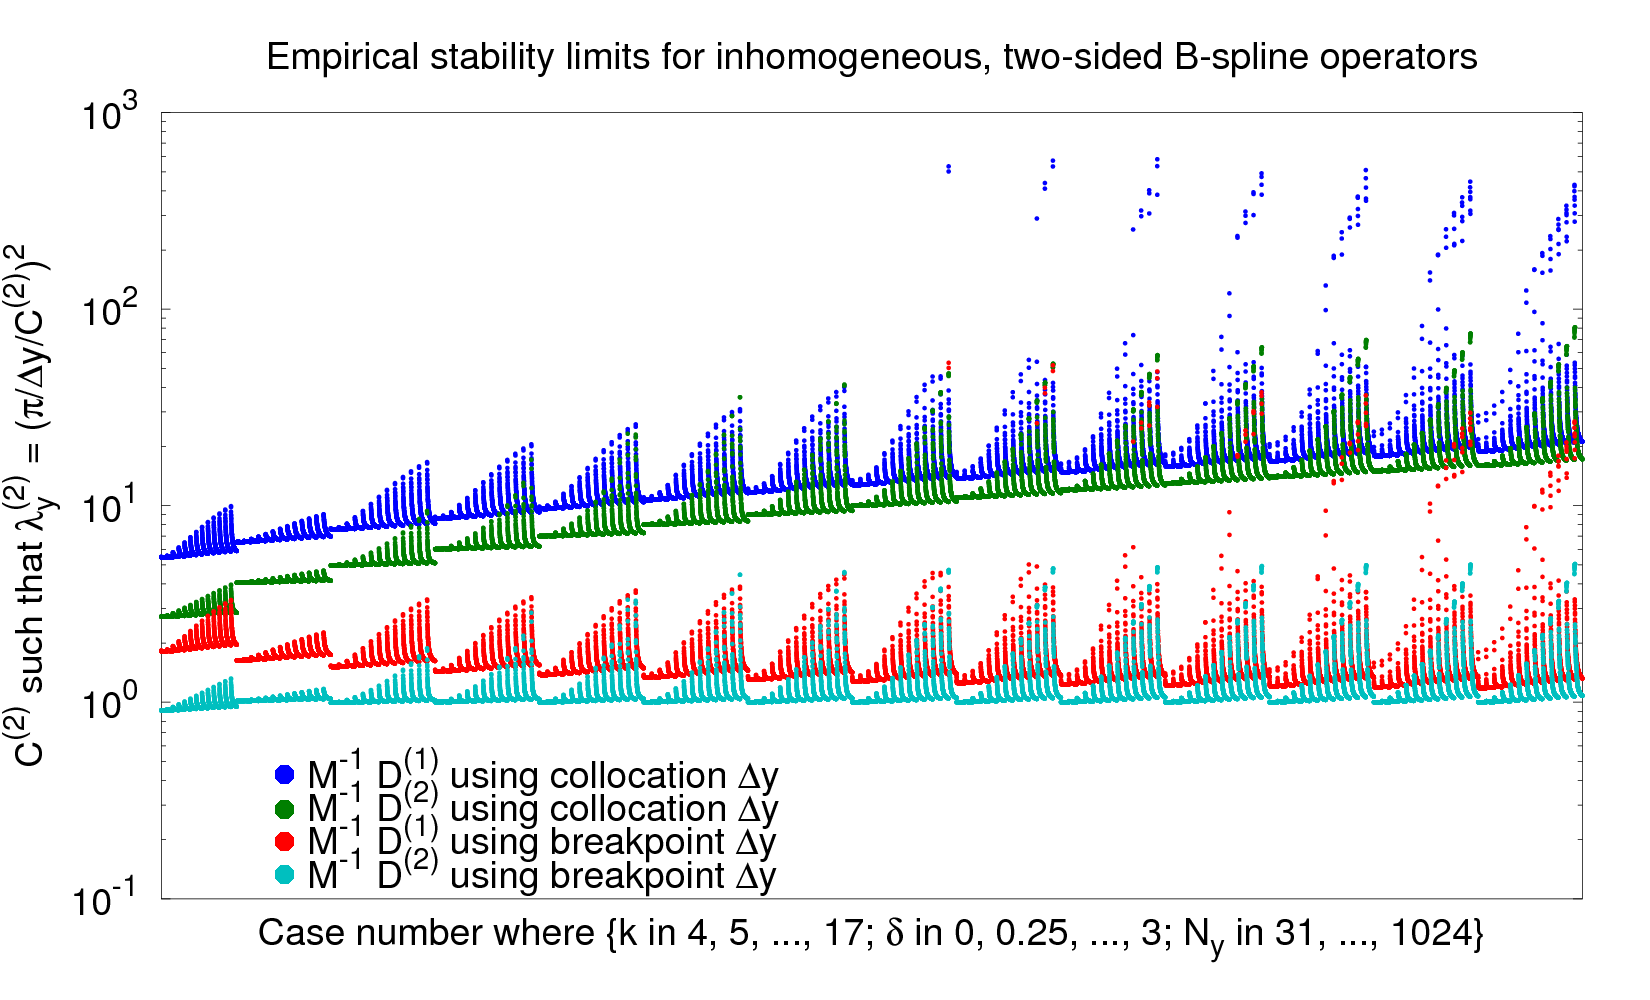
\includegraphics[width=5.5in]{inhomogeneity2}
  \\
  \vspace{0.5em}
  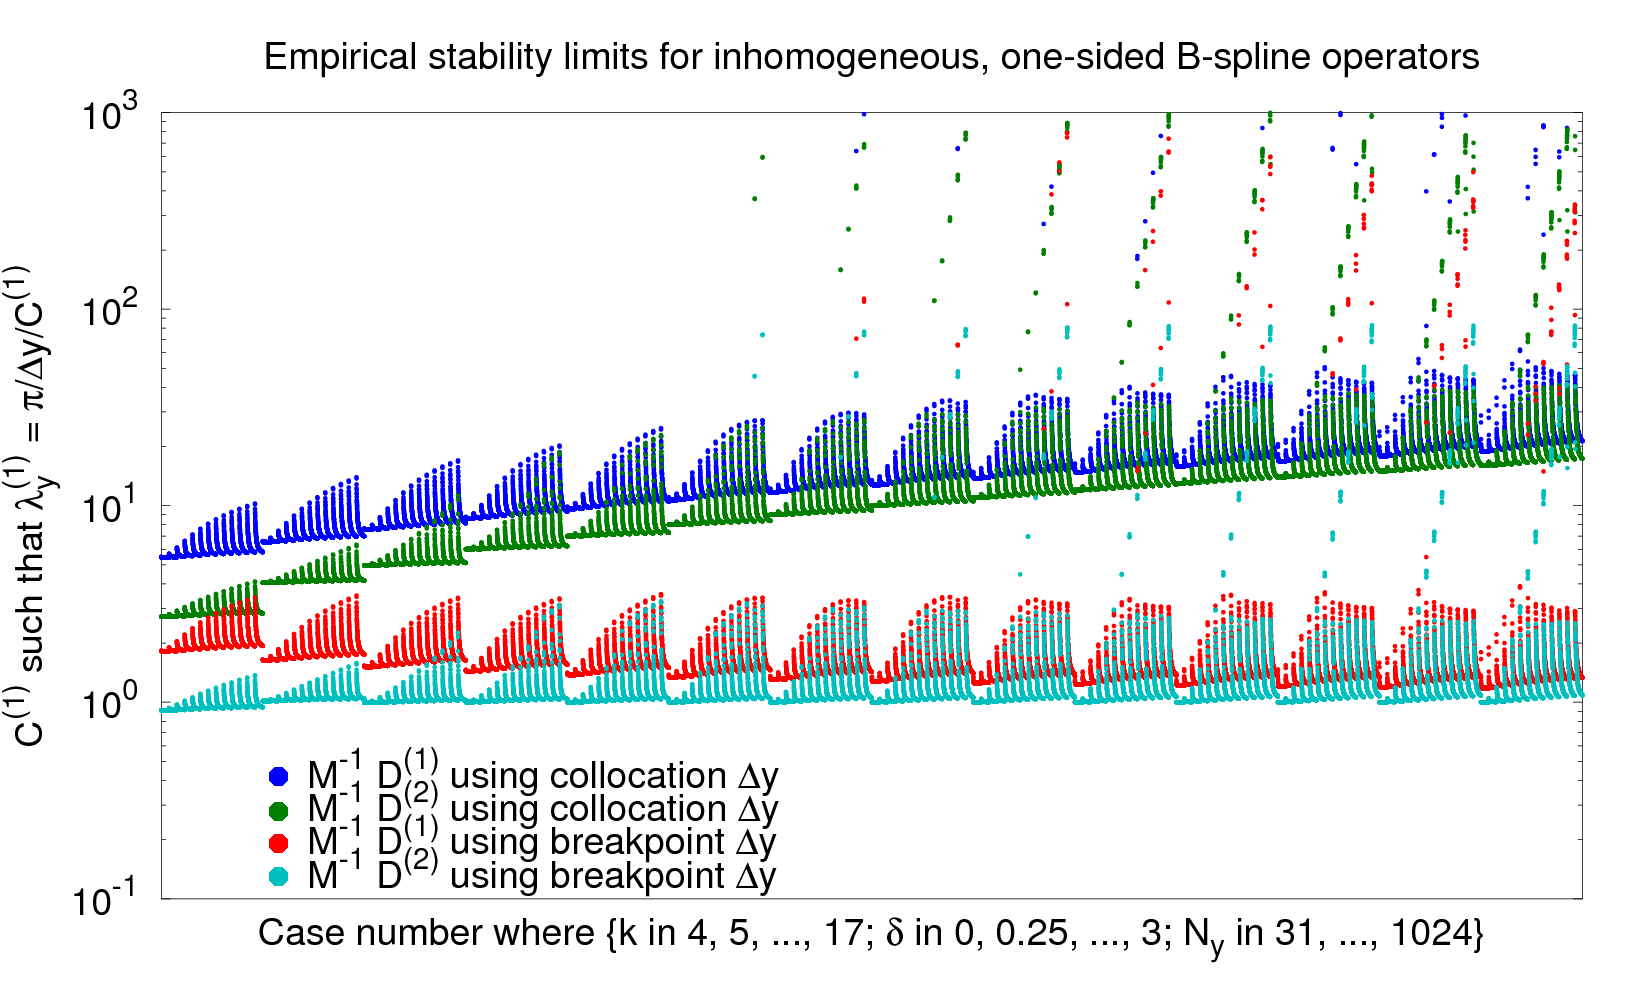
\includegraphics[width=5.5in]{inhomogeneity1}
  \\
  \caption[Exact maximum eigenvalues for inhomogeneous B-spline operators]{%
  Exact values of $C^{(1)}$ and $C^{(2)}$ computed per
  Equations~\eqref{eq:lambda1deltay} and~\eqref{eq:lambda2deltay} for roughly
  32,500 combinations of $k$, $\delta$, and $N_y$.  Above, two-sided stretching
  was performed on breakpoints per~\eqref{eq:htstretch2}.  Below, one-sided
  stretching was performed per~\eqref{eq:htstretch1}.  In both figures, the
  leftmost four ``triangles'' correspond to $k=4$ while $\delta$ was varied
  slowly and $N_y$ varied quickly.  Moving rightward, the next ``triangles''
  are for $k=5$, then $k=6$, etc.
  \label{fig:inhomogeneity}
  }
\end{figure}

Using numerically obtained eigenvalue magnitudes
$\lambda^{(1)}=\lambda^{(1)}_y\!\left(k,\delta,N_y\right)$ and
$\lambda^{(2)}=\lambda^{(2)}_y\!\left(k,\delta,N_y\right)$ from a large
collection of discrete operators, exact $C^{(1)}$ and $C^{(2)}$ values were
computed.  The results are shown in \autoref{fig:inhomogeneity}.  The minimum
grid spacing $\Delta{}y$ was measured using either adjacent breakpoints or
adjacent collocation points to permit a comparison.  Considering only
breakpoint-based results for $k=8$, one can see how \citet{Venugopal2003}
probably chose $C^{(1)}=4$ and $C^{(2)}=1$ as discussed in
\autoref{sec:convectivestability} and \autoref{sec:diffusivestability}.
However, it is striking just how nonuniversal those choices are.
Evidently, neither a breakpoint-based nor a collocation point-based $\Delta{}y$
inherently captures the maximum eigenvalue magnitudes as $k$, $\delta$, and
$N_y$ vary--- some nonlinear combination of the complete set of grid parameters
is necessary.

Hereafter, unlike \citeauthor{Guarini1998}, \citeauthor{Kwok2002}, and
\citeauthor{Venugopal2003}, we take $\Delta{}y$ to be the spacing between
adjacent collocation points.  Performing Levenberg--Marquardt nonlinear
regression against the vast majority of the empirical data in
\autoref{fig:inhomogeneity} shows good agreement with curve fits like the
following
\begin{subequations}
\begin{align}
  \label{eq:Cfit}
  C_\text{approx}^{(i)}\!\left(k,\delta,N_y\right)
  &\approx
    a k
  + b \hat\delta
  + \frac{c}{\sqrt{k}}
  + k^{d + e \hat\delta} \left(
        1 + \left(\frac{f k}{N_y - k + 1}\right)^{g k + h \hat\delta}
    \right)
  ,
  \\
  \hat\delta &= \left(1+\delta\right)^i \tanh \delta.
\end{align}
\end{subequations}
The data from ``nearly spectral'' discrete operators, defined as when $N_y \leq
5 k$, proved difficult to fit and was omitted.  Such cases look like outliers
in \autoref{fig:inhomogeneity} and are not operationally important as
the present work does not use a spectral wall-normal basis.  When
using two-sided stretching per~\eqref{eq:htstretch2}, one collection of
constants $a$--$i$ permits fitting the retained $C^{(1)}$ observations for
$k=5$ through $11$ to within relative errors of [-2.55\%, 1.76\%].  Another
collection permits fitting retained $C^{(2)}$ observations to within [-11.3\%,
17.1\%].  While those results are encouraging for the generality of the chosen
functional forms, they are less than satisfactory for production use.  More
precise, $k$-specific, coefficients for two-sided stretching appear in
\autoref{tab:C1fit2} and \autoref{tab:C2fit2} while coefficients for one-sided
stretching appear in \autoref{tab:C1fit1} and \autoref{tab:C2fit1}.

Unfortunately, using either $C_\text{approx}^{(1)}$ or $C_\text{approx}^{(2)}$
directly proved to be overly aggressive as measured using a collection of
contrived test problems known \emph{a priori} to be either convectively or
diffusively limited.  Scaling these by a single safety factor was problematic as no
unique value allowed pushing up against both criteria simultaneously.  Against
the same test problems, however, using approximations like the square root of
$C_\text{approx}^{(i)}$ did permit using a uniform safety factor across a
variety of test conditions.

In summary, the present work takes nearly the square root of a conservative
estimate of $C_\text{approx}^{(i)}$.  That is,
\begin{align}
  C^{(1)} &= \left(
      \frac{C_\text{approx}^{(1)}}
           {1 - \text{(negative relative error percentage)}/100}
  \right)^{33/64}
\\
  C^{(2)} &= \left(
      \frac{C_\text{approx}^{(2)}}
           {1 - \text{(negative relative error percentage)}/100}
  \right)^{27/64}
\end{align}
where the fit-specific, negative-valued lower error bounds appear in the
rightmost column of the coefficient tables.  Adjusting to the empirical fits'
lower bounds gives slightly more conservative $\lambda_y^{(i)}$ estimates.  These
values of $C^{(i)}$ are plugged into Equations~\eqref{eq:lambda1deltay}
and~\eqref{eq:lambda2deltay} with those results feeding into
Equations~\eqref{eq:convectivestability} and~\eqref{eq:diffusivestability}.
These estimates were designed for use with safety factors like 0.72 whenever
$N_y > 5k$,  which will be revisited in
\autoref{sec:channel_runs}.

\begin{sidewaystable}
\centering
\caption[
    B-spline order-specific curve fits for $C_\text{approx}^{(1)}$
    for stretching~\eqref{eq:htstretch2}.
]{%
    B-spline order-specific curve fits for estimating $C_\text{approx}^{(1)}$
    via Equation~\eqref{eq:Cfit} when $\Delta{}y$ is the minimum distance
    between \emph{collocation points} from breakpoints stretched according
    to $f_2$ defined in~\eqref{eq:htstretch2}.
}
\label{tab:C1fit2}
\vspace{1em}
\renewcommand{\arraystretch}{1.40}   % Adds whitespace between rows
\begin{tabular}{r|ccccccccc|c@{ -- }c@{\%}}
 $k$ & $a$ & $b$ & $c$ & $d$ & $e$ & $f$ & $g$ & $h$ & $i$
     & \multicolumn{2}{c}{relative error}
\\ \hline
%%%%%%%%%%
% TWOSIDED
%%%%%%%%%%
5--11
&  $\frac{            5054}{            4549}$
& -$\frac{            3953}{           12175}$
&  $\frac{            4321}{            5893}$
& -$\frac{            5839}{            8805}$
&  $\frac{            3121}{            7385}$
&  $\frac{          235081}{            5659}$
&  $\frac{             399}{           13421}$
&  $\frac{            2795}{            8687}$
&  $\frac{            3548}{            7037}$
&  -2.55 &  1.76
\\
4
&  $\frac{            8753}{            6138}$
&  $\frac{             184}{            3513}$
& -$\frac{            3868}{            6327}$
& -$\frac{           22756}{            5215}$
&  $\frac{           19435}{           28258}$
&  $\frac{       152882005}{            9731}$
&  $\frac{            1605}{           12298}$
&  $\frac{             814}{            5783}$
&  $\frac{            7755}{           19621}$
&  -1.52 &  0.46
\\
5
& -$\frac{          182723}{            7970}$
&  $\frac{             121}{            6080}$
& -$\frac{         7061095}{           23119}$
&  $\frac{          115483}{           33477}$
&  $\frac{               1}{            5560}$
&  $\frac{             197}{            3683}$
&  $\frac{             761}{            2741}$
& -$\frac{            2307}{            6251}$
&  $\frac{            1845}{            5548}$
&  -1.12 &  0.53
\\
6
&  $\frac{            8193}{            7183}$
&  $\frac{              74}{            7487}$
&  $\frac{           10787}{            6960}$
& -$\frac{           12529}{            6209}$
&  $\frac{            3196}{            4771}$
&  $\frac{         4441318}{           12819}$
&  $\frac{             932}{           12135}$
&  $\frac{            3915}{           17923}$
&  $\frac{             870}{            2123}$
&  -1.39 &  1.14
\\
7
&  $\frac{            9063}{            5683}$
&  $\frac{             291}{            6739}$
& -$\frac{           26786}{            3839}$
& -$\frac{            2757}{            1352}$
&  $\frac{            2959}{            4613}$
&  $\frac{         2666741}{            4919}$
&  $\frac{             507}{            6947}$
&  $\frac{             498}{            2627}$
&  $\frac{            3572}{            8791}$
&  -1.50 &  1.12
\\
8
&  $\frac{           20956}{           18111}$
&  $\frac{              73}{            3043}$
&  $\frac{            3316}{            4207}$
& -$\frac{           17945}{           10877}$
&  $\frac{            6659}{           11166}$
&  $\frac{         2564433}{            9169}$
&  $\frac{             658}{           10813}$
&  $\frac{            2725}{           12594}$
&  $\frac{            1181}{            2847}$
&  -1.48 &  1.18
\\
9
&  $\frac{            4351}{            3996}$
&  $\frac{             204}{            4093}$
&  $\frac{           13726}{            5957}$
& -$\frac{           19388}{           12047}$
&  $\frac{           10397}{           18003}$
&  $\frac{         1200048}{            3823}$
&  $\frac{             246}{            4289}$
&  $\frac{            1395}{            6839}$
&  $\frac{            4244}{           10183}$
&  -1.54 &  1.09
\\
10
&  $\frac{            3174}{            3221}$
&  $\frac{             340}{            4047}$
&  $\frac{          435835}{           78898}$
& -$\frac{           24457}{           14830}$
&  $\frac{            3057}{            5416}$
&  $\frac{         5464428}{           12505}$
&  $\frac{             166}{            3013}$
&  $\frac{             679}{            3691}$
&  $\frac{            2669}{            6422}$
&  -1.59 &  1.11
\\
11
&  $\frac{            6141}{            6356}$
&  $\frac{             513}{            5051}$
&  $\frac{           35557}{            5371}$
& -$\frac{            5359}{            3384}$
&  $\frac{            6824}{           12279}$
&  $\frac{         3628675}{            8504}$
&  $\frac{            1012}{           19681}$
&  $\frac{             363}{            2008}$
&  $\frac{            1873}{            4520}$
&  -1.56 &  0.94
\\
12
&  $\frac{            9953}{            8604}$
&  $\frac{             521}{            4751}$
& -$\frac{            2623}{            3140}$
& -$\frac{           12011}{            8190}$
&  $\frac{            9067}{           16522}$
&  $\frac{         1947584}{            5723}$
&  $\frac{             141}{            2959}$
&  $\frac{            1231}{            6652}$
&  $\frac{            8479}{           20445}$
&  -1.58 &  1.12
\\
13
&  $\frac{            6428}{            6247}$
&  $\frac{              28}{             239}$
&  $\frac{           28437}{            6178}$
& -$\frac{           13912}{           10071}$
&  $\frac{            2717}{            5125}$
&  $\frac{         3512083}{           11082}$
&  $\frac{             542}{           12275}$
&  $\frac{             701}{            3776}$
&  $\frac{            7291}{           17441}$
&  -1.58 &  1.08
\\
14
&  $\frac{           18221}{           17050}$
&  $\frac{             573}{            3767}$
&  $\frac{           37351}{           13944}$
& -$\frac{           12384}{            8881}$
&  $\frac{            2238}{            4193}$
&  $\frac{         3701821}{           10597}$
&  $\frac{             231}{            5389}$
&  $\frac{            2953}{           16836}$
&  $\frac{            3950}{            9507}$
&  -1.59 &  1.10
\\
15
&  $\frac{            9251}{            9369}$
&  $\frac{            1001}{            5400}$
&  $\frac{         1033331}{          141480}$
& -$\frac{           13367}{            9358}$
&  $\frac{            7583}{           14554}$
&  $\frac{         2662722}{            5819}$
&  $\frac{             392}{            9519}$
&  $\frac{             555}{            3394}$
&  $\frac{            2181}{            5234}$
&  -1.56 &  1.01
\\
16
&  $\frac{            8003}{            8200}$
&  $\frac{            2503}{           12108}$
&  $\frac{          263686}{           31457}$
& -$\frac{            5713}{            4107}$
&  $\frac{            4803}{            9290}$
&  $\frac{         8189082}{           18419}$
&  $\frac{              93}{            2371}$
&  $\frac{            1663}{           10299}$
&  $\frac{            2945}{            7073}$
&  -1.56 &  1.08
\\
17
&  $\frac{           10594}{            8835}$
&  $\frac{            2615}{           11361}$
& -$\frac{           38602}{            5641}$
& -$\frac{            3464}{            2537}$
&  $\frac{            3372}{            6575}$
&  $\frac{         4481119}{           10024}$
&  $\frac{             355}{            9469}$
&  $\frac{             811}{            5107}$
&  $\frac{            1129}{            2714}$
&  -1.53 &  0.97
\end{tabular}
\end{sidewaystable}

\begin{sidewaystable}
\centering
\caption[
    B-spline order-specific curve fits for $C_\text{approx}^{(1)}$
    for stretching~\eqref{eq:htstretch1}.
]{%
    B-spline order-specific curve fits for estimating $C_\text{approx}^{(1)}$
    via Equation~\eqref{eq:Cfit} when $\Delta{}y$ is the minimum distance
    between \emph{collocation points} from breakpoints stretched according
    to $f_1$ defined in~\eqref{eq:htstretch1}.
}
\label{tab:C1fit1}
\vspace{1em}
\renewcommand{\arraystretch}{1.40}   % Adds whitespace between rows
\begin{tabular}{r|ccccccccc|c@{ -- }c@{\%}}
 $k$ & $a$ & $b$ & $c$ & $d$ & $e$ & $f$ & $g$ & $h$ & $i$
     & \multicolumn{2}{c}{relative error}
\\ \hline
%%%%%%%%%%
% ONESIDED
%%%%%%%%%%
5--11
&  $\frac{           12101}{           11060}$
& -$\frac{           16426}{           49749}$
&  $\frac{            4524}{           12157}$
& -$\frac{            4083}{            8722}$
&  $\frac{            4648}{           11133}$
&  $\frac{          645696}{           14887}$
&  $\frac{             117}{            4057}$
&  $\frac{            3436}{            8883}$
&  $\frac{            2329}{            6500}$
&  -2.80 &  2.67
\\
4
&  $\frac{            4129}{            3316}$
&  $\frac{            1052}{           13345}$
&  $\frac{            5769}{            7262}$
& -$\frac{           29140}{            6539}$
&  $\frac{            3051}{            5753}$
&  $\frac{       271951060}{            6969}$
&  $\frac{            3691}{           26472}$
&  $\frac{             458}{            3255}$
&  $\frac{            3944}{           13269}$
&  -2.65 &  1.39
\\
5
&  $\frac{            3747}{            2863}$
&  $\frac{             722}{            6223}$
& -$\frac{            3064}{           13069}$
& -$\frac{           43215}{           13954}$
&  $\frac{            4867}{            8717}$
&  $\frac{        54938146}{           12669}$
&  $\frac{             607}{            5225}$
&  $\frac{             863}{            5306}$
&  $\frac{            1663}{            5196}$
&  -2.73 &  1.43
\\
6
&  $\frac{             793}{             577}$
&  $\frac{            2234}{           16675}$
& -$\frac{           12137}{            6441}$
& -$\frac{           19450}{            5421}$
&  $\frac{            8944}{           17333}$
&  $\frac{       201430625}{            6661}$
&  $\frac{             799}{            7654}$
&  $\frac{            1290}{            9821}$
&  $\frac{             974}{            3283}$
&  -3.00 &  1.48
\\
7
&  $\frac{           10401}{            9794}$
&  $\frac{            1356}{            8845}$
&  $\frac{           30469}{           10756}$
& -$\frac{           11151}{            3473}$
&  $\frac{            3321}{            7345}$
&  $\frac{      1029376385}{           36246}$
&  $\frac{             377}{            4242}$
&  $\frac{            1838}{           13631}$
&  $\frac{            2446}{            8123}$
&  -2.88 &  1.50
\\
8
&  $\frac{           13867}{           11300}$
&  $\frac{            1847}{           10004}$
& -$\frac{             899}{            1084}$
& -$\frac{           24247}{            8311}$
&  $\frac{            2025}{            4691}$
&  $\frac{       208465759}{            9898}$
&  $\frac{            1195}{           15107}$
&  $\frac{             131}{             957}$
&  $\frac{            3041}{            9933}$
&  -2.90 &  1.47
\\
9
&  $\frac{           11292}{           11417}$
&  $\frac{            2667}{           12475}$
&  $\frac{           71783}{           14593}$
& -$\frac{           23753}{            8884}$
&  $\frac{           15279}{           38327}$
&  $\frac{       170388497}{           10015}$
&  $\frac{             913}{           12919}$
&  $\frac{            2803}{           19841}$
&  $\frac{           16957}{           54130}$
&  -2.87 &  1.41
\\
10
&  $\frac{            4941}{            9610}$
&  $\frac{             830}{            3611}$
&  $\frac{          279834}{           13813}$
& -$\frac{            4892}{            2245}$
&  $\frac{            1823}{            4351}$
&  $\frac{        11323441}{            2063}$
&  $\frac{             366}{            5827}$
&  $\frac{            1918}{           12879}$
&  $\frac{            2981}{            9362}$
&  -2.83 &  1.42
\\
11
&  $\frac{           12725}{           12639}$
&  $\frac{            1233}{            4685}$
&  $\frac{           29103}{            5882}$
& -$\frac{           17641}{            7391}$
&  $\frac{             812}{            2251}$
&  $\frac{        93817310}{            6013}$
&  $\frac{             575}{            9852}$
&  $\frac{            1238}{            8665}$
&  $\frac{            2801}{            8822}$
&  -2.79 &  1.32
\\
12
&  $\frac{            5215}{            5156}$
&  $\frac{            1009}{            3470}$
&  $\frac{           77977}{           15613}$
& -$\frac{           29719}{           12774}$
&  $\frac{            3890}{           10879}$
&  $\frac{        75236231}{            4566}$
&  $\frac{             579}{           10655}$
&  $\frac{            3977}{           28471}$
&  $\frac{            2948}{            9301}$
&  -2.86 &  1.36
\\
13
&  $\frac{           16753}{           16972}$
&  $\frac{             794}{            2485}$
&  $\frac{          100717}{           15948}$
& -$\frac{           34434}{           15637}$
&  $\frac{            2493}{            7441}$
&  $\frac{        61372987}{            4090}$
&  $\frac{             479}{            9560}$
&  $\frac{             451}{            3156}$
&  $\frac{            1286}{            3991}$
&  -2.82 &  1.34
\\
14
&  $\frac{            9761}{            9871}$
&  $\frac{            1461}{            4217}$
&  $\frac{             281}{              43}$
& -$\frac{           33703}{           15770}$
&  $\frac{            6378}{           19271}$
&  $\frac{       170777218}{           11389}$
&  $\frac{             543}{           11569}$
&  $\frac{            1880}{           13293}$
&  $\frac{            4685}{           14541}$
&  -2.82 &  1.33
\\
15
&  $\frac{            7329}{            7286}$
&  $\frac{            2281}{            6042}$
&  $\frac{           48733}{            8398}$
& -$\frac{            8421}{            4222}$
&  $\frac{            1839}{            6014}$
&  $\frac{        87107021}{            7039}$
&  $\frac{            1578}{           36371}$
&  $\frac{            1153}{            7805}$
&  $\frac{            1189}{            3613}$
&  -2.72 &  1.29
\\
16
&  $\frac{            7733}{            8163}$
&  $\frac{            3533}{            8665}$
&  $\frac{          121822}{           12527}$
& -$\frac{            6932}{            3573}$
&  $\frac{            2407}{            8036}$
&  $\frac{        57224710}{            4651}$
&  $\frac{             286}{            6989}$
&  $\frac{             377}{            2558}$
&  $\frac{            4584}{           13895}$
&  -2.72 &  1.29
\\
17
&  $\frac{           10349}{            9079}$
&  $\frac{            4121}{            9390}$
& -$\frac{           49628}{           15233}$
& -$\frac{           16811}{            8933}$
&  $\frac{            1143}{            3880}$
&  $\frac{       103494425}{            8753}$
&  $\frac{            1589}{           41049}$
&  $\frac{             817}{            5544}$
&  $\frac{            2196}{            6637}$
&  -2.66 &  1.24
\end{tabular}
\end{sidewaystable}

\begin{sidewaystable}
\centering
\caption[
    B-spline order-specific curve fits for $C_\text{approx}^{(2)}$
    for stretching~\eqref{eq:htstretch2}.
]{%
    B-spline order-specific curve fits for estimating $C_\text{approx}^{(2)}$
    via Equation~\eqref{eq:Cfit} when $\Delta{}y$ is the minimum distance
    between \emph{collocation points} from breakpoints stretched according
    to $f_2$ defined in~\eqref{eq:htstretch2}.
}
\label{tab:C2fit2}
\vspace{1em}
\renewcommand{\arraystretch}{1.40}   % Adds whitespace between rows
\begin{tabular}{r|ccccccccc|c@{ -- }c@{\%}}
 $k$ & $a$ & $b$ & $c$ & $d$ & $e$ & $f$ & $g$ & $h$ & $i$
     & \multicolumn{2}{c}{relative error}
\\ \hline
%%%%%%%%%%
% TWOSIDED
%%%%%%%%%%
5--11
&  $\frac{            5958}{            6049}$
&  $\frac{             334}{            5909}$
& -$\frac{           14563}{            5926}$
& -$\frac{           35330}{           11929}$
&  $\frac{            1554}{            3265}$
&  $\frac{         4042664}{            8379}$
&  $\frac{             887}{            9011}$
&  $\frac{            2243}{           13757}$
&  $\frac{            1066}{            1585}$
&  -11.30 &  17.11
\\
4
& -$\frac{          132683}{            8121}$
& -$\frac{               8}{            7617}$
& -$\frac{         1156372}{            9759}$
&  $\frac{           78080}{           22333}$
&  $\frac{               2}{           10139}$
&  $\frac{              83}{            5144}$
&  $\frac{             911}{            2744}$
& -$\frac{            4791}{           13862}$
&  $\frac{            1479}{            4412}$
&  -1.86 &  1.81
\\
5
& -$\frac{           96752}{           19419}$
&  $\frac{              27}{           10108}$
& -$\frac{          360604}{            4723}$
&  $\frac{           24551}{            9533}$
&  $\frac{               1}{            5309}$
&  $\frac{             277}{            4330}$
&  $\frac{           13424}{           46671}$
& -$\frac{            3888}{           10265}$
&  $\frac{            1289}{            3770}$
&  -0.50 &  0.32
\\
6
&  $\frac{            2635}{            8541}$
& -$\frac{             299}{           15112}$
&  $\frac{          174058}{           24237}$
& -$\frac{           17342}{           13001}$
&  $\frac{            2894}{           10471}$
&  $\frac{          291982}{            9057}$
&  $\frac{              68}{           17203}$
&  $\frac{            5579}{           13080}$
&  $\frac{            6911}{            9355}$
&  -1.51 &  2.62
\\
7
&  $\frac{            7358}{           11623}$
& -$\frac{             120}{            6169}$
&  $\frac{           82091}{           23515}$
& -$\frac{           10147}{            9621}$
&  $\frac{            2735}{           11778}$
&  $\frac{          212175}{            7154}$
&  $\frac{              10}{            6231}$
&  $\frac{           10354}{           24479}$
&  $\frac{            2416}{            3043}$
&  -1.70 &  3.97
\\
8
&  $\frac{            4751}{            5346}$
&  $\frac{            2143}{           18802}$
& -$\frac{           46259}{           19493}$
& -$\frac{            4506}{            9193}$
&  $\frac{               4}{            6951}$
&  $\frac{           49249}{            1482}$
& -$\frac{              24}{            8359}$
&  $\frac{             959}{            3662}$
&  $\frac{            9327}{            7114}$
&  -4.50 &  6.86
\\
9
&  $\frac{           17841}{           19519}$
&  $\frac{             553}{            8538}$
& -$\frac{           20719}{            8083}$
& -$\frac{            3783}{            7057}$
&  $\frac{             856}{           10529}$
&  $\frac{          121124}{            5101}$
& -$\frac{             115}{           30303}$
&  $\frac{            2467}{            7116}$
&  $\frac{            4707}{            4139}$
&  -3.68 &  7.17
\\
10
&  $\frac{           20122}{            5145}$
& -$\frac{               5}{            6272}$
& -$\frac{         1003532}{           10415}$
& -$\frac{           11287}{           15030}$
&  $\frac{            3429}{           17696}$
&  $\frac{          258125}{            9817}$
&  $\frac{               7}{            7694}$
&  $\frac{            4286}{            9151}$
&  $\frac{            8126}{            9217}$
&  -5.97 &  8.01
\\
11
&  $\frac{           32624}{           11799}$
&  $\frac{              23}{            3905}$
& -$\frac{          466211}{            6855}$
& -$\frac{           14065}{           10992}$
&  $\frac{            4693}{           11010}$
&  $\frac{          335615}{            7641}$
&  $\frac{             187}{            7994}$
&  $\frac{            4512}{            8461}$
&  $\frac{            1469}{            2419}$
&  -6.09 &  6.61
\\
12
&  $\frac{           21510}{           19531}$
&  $\frac{             407}{            3029}$
& -$\frac{           40991}{            5317}$
& -$\frac{           34333}{           13993}$
&  $\frac{            7253}{            9181}$
&  $\frac{         1291629}{            5929}$
&  $\frac{             217}{            3456}$
&  $\frac{            2659}{            8092}$
&  $\frac{            4103}{            9334}$
&  -6.88 &  6.21
\\
13
&  $\frac{            3889}{            5285}$
&  $\frac{            2389}{           15117}$
&  $\frac{           52947}{            6029}$
& -$\frac{           17456}{            5339}$
&  $\frac{            4061}{            4625}$
&  $\frac{        11135709}{            8452}$
&  $\frac{             488}{            7087}$
&  $\frac{            1474}{            6209}$
&  $\frac{             383}{             987}$
&  -6.88 &  5.89
\\
14
&  $\frac{           13010}{           10487}$
&  $\frac{            1375}{           10628}$
& -$\frac{          201367}{           12385}$
& -$\frac{           24232}{            6743}$
&  $\frac{           11512}{           10801}$
&  $\frac{         6297203}{            2487}$
&  $\frac{             428}{            6171}$
&  $\frac{             648}{            3823}$
&  $\frac{            4064}{           11831}$
&  -6.54 &  5.79
\\
15
&  $\frac{           25912}{           21893}$
&  $\frac{            1831}{           16699}$
& -$\frac{           58570}{            4063}$
& -$\frac{           14377}{            4017}$
&  $\frac{           18889}{           18281}$
&  $\frac{        16561349}{            4390}$
&  $\frac{             272}{            4179}$
&  $\frac{             367}{            2451}$
&  $\frac{             919}{            2686}$
&  -6.57 &  5.36
\\
16
&  $\frac{            3826}{            5191}$
&  $\frac{             800}{           13057}$
&  $\frac{          213790}{           16397}$
& -$\frac{           16873}{            4447}$
&  $\frac{           10559}{            9248}$
&  $\frac{        84802177}{           11958}$
&  $\frac{             607}{            9491}$
&  $\frac{            1313}{           14052}$
&  $\frac{            2667}{            8263}$
&  -6.11 &  5.04
\\
17
&  $\frac{            6127}{            6960}$
& -$\frac{             163}{            9791}$
&  $\frac{           22545}{            4961}$
& -$\frac{          115738}{           31923}$
&  $\frac{           10232}{           10879}$
&  $\frac{       167869433}{           10467}$
&  $\frac{             439}{            8114}$
&  $\frac{           10720}{           81537}$
&  $\frac{            3302}{           10275}$
&  -5.35 &  4.96
\end{tabular}
\end{sidewaystable}

\begin{sidewaystable}
\centering
\caption[
    B-spline order-specific curve fits for $C_\text{approx}^{(2)}$
    for stretching~\eqref{eq:htstretch1}.
]{%
    B-spline order-specific curve fits for estimating $C_\text{approx}^{(2)}$
    via Equation~\eqref{eq:Cfit} when $\Delta{}y$ is the minimum distance
    between \emph{collocation points} from breakpoints stretched according to
    $f_1$ defined in~\eqref{eq:htstretch1}.
}
\label{tab:C2fit1}
\vspace{1em}
\renewcommand{\arraystretch}{1.40}   % Adds whitespace between rows
\begin{tabular}{r|ccccccccc|c@{ -- }c@{\%}}
 $k$ & $a$ & $b$ & $c$ & $d$ & $e$ & $f$ & $g$ & $h$ & $i$
     & \multicolumn{2}{c}{relative error}
\\ \hline
%%%%%%%%%%
% ONESIDED
%%%%%%%%%%
5--11
&  $\frac{           10951}{           10966}$
&  $\frac{             692}{           17487}$
& -$\frac{           58794}{           21577}$
& -$\frac{           12439}{            4860}$
&  $\frac{            1536}{            1951}$
&  $\frac{         1826729}{            9846}$
&  $\frac{             854}{            8115}$
&  $\frac{            1731}{            7739}$
&  $\frac{            2360}{            5791}$
&  -23.87 &  19.78
\\
4
& -$\frac{           37181}{            3006}$
& -$\frac{              35}{           19004}$
& -$\frac{         1709799}{           12403}$
&  $\frac{           11429}{            3303}$
&  $\frac{               1}{            4633}$
&  $\frac{             207}{            9529}$
&  $\frac{            8025}{           25267}$
& -$\frac{            1792}{            5289}$
&  $\frac{            1579}{            6332}$
&  -2.73 &  2.66
\\
5
&  $\frac{            6843}{            7364}$
& -$\frac{             113}{            5126}$
& -$\frac{           19508}{           11693}$
& -$\frac{           15410}{            9853}$
&  $\frac{            2215}{            5596}$
&  $\frac{          199827}{            5060}$
&  $\frac{             117}{            5482}$
&  $\frac{            3886}{            7977}$
&  $\frac{            3618}{            7763}$
&  -0.63 &  1.38
\\
6
&  $\frac{            1309}{            1894}$
&  $\frac{             472}{            6839}$
&  $\frac{           10796}{           10079}$
& -$\frac{           13268}{           14331}$
&  $\frac{            1942}{           14501}$
&  $\frac{          169657}{            5987}$
&  $\frac{               2}{            3287}$
&  $\frac{            1786}{            3447}$
&  $\frac{            9664}{           13071}$
&  -3.14 &  5.22
\\
7
&  $\frac{           62991}{           64619}$
&  $\frac{           10271}{           61625}$
& -$\frac{          146725}{           39021}$
& -$\frac{            6349}{           10362}$
&  $\frac{              23}{            3440}$
&  $\frac{           26371}{             794}$
& -$\frac{              17}{           10006}$
&  $\frac{             798}{            1681}$
&  $\frac{           13080}{           14621}$
&  -4.53 &  9.31
\\
8
&  $\frac{            5701}{            6404}$
&  $\frac{             543}{           10115}$
& -$\frac{           15926}{           10845}$
& -$\frac{            9214}{           11799}$
&  $\frac{            1960}{            8807}$
&  $\frac{          759503}{           31646}$
&  $\frac{               9}{            4685}$
&  $\frac{            3636}{            5393}$
&  $\frac{            5996}{            8919}$
&  -5.10 &  7.39
\\
9
&  $\frac{           57103}{           12153}$
&  $\frac{             349}{            6313}$
& -$\frac{          292899}{            2840}$
& -$\frac{           15197}{           10802}$
&  $\frac{            3317}{            6840}$
&  $\frac{         6115361}{          140104}$
&  $\frac{             431}{            8216}$
&  $\frac{            7073}{           12325}$
&  $\frac{           10286}{           21381}$
&  -6.57 &  7.12
\\
10
&  $\frac{            4753}{            6483}$
&  $\frac{             215}{            1719}$
&  $\frac{           32327}{            6251}$
& -$\frac{            8563}{            4452}$
&  $\frac{            1981}{            2831}$
&  $\frac{         1180287}{           14438}$
&  $\frac{             599}{            7682}$
&  $\frac{            1695}{            4003}$
&  $\frac{            3259}{            8267}$
&  -8.44 &  6.56
\\
11
&  $\frac{            3058}{            4871}$
&  $\frac{            2994}{           14713}$
&  $\frac{           34703}{            3382}$
& -$\frac{           15557}{            4053}$
&  $\frac{            6541}{            5144}$
&  $\frac{         5024384}{            5503}$
&  $\frac{            2720}{           22829}$
&  $\frac{             961}{           20910}$
&  $\frac{            2347}{            7629}$
&  -6.87 &  7.13
\\
12
&  $\frac{           12242}{           10351}$
&  $\frac{             785}{            5066}$
& -$\frac{          108847}{            9907}$
& -$\frac{           38407}{            8945}$
&  $\frac{            8189}{            5423}$
&  $\frac{        54739986}{           21557}$
&  $\frac{            1903}{           16894}$
& -$\frac{             381}{            7330}$
&  $\frac{            6661}{           24933}$
&  -7.21 &  7.11
\\
13
&  $\frac{           24826}{           20307}$
&  $\frac{            4749}{           40912}$
& -$\frac{          170233}{           12219}$
& -$\frac{            4785}{            1084}$
&  $\frac{           16494}{           11557}$
&  $\frac{       720241352}{          105099}$
&  $\frac{            2930}{           29579}$
& -$\frac{             807}{           19174}$
&  $\frac{            2725}{           10439}$
&  -7.16 &  6.65
\\
14
&  $\frac{           13245}{           12827}$
&  $\frac{             163}{            5022}$
& -$\frac{           25753}{            4855}$
& -$\frac{          176237}{           37876}$
&  $\frac{           21379}{           17208}$
&  $\frac{       315490949}{            7639}$
&  $\frac{            4100}{           49413}$
&  $\frac{               2}{            4983}$
&  $\frac{            1942}{            7671}$
&  -6.65 &  6.31
\\
15
&  $\frac{            5358}{            5287}$
& -$\frac{             142}{           11949}$
& -$\frac{           16365}{            3631}$
& -$\frac{          173358}{           39355}$
&  $\frac{           10908}{           10097}$
&  $\frac{       529204799}{            8657}$
&  $\frac{             119}{            1628}$
&  $\frac{             216}{            7747}$
&  $\frac{            1637}{            6397}$
&  -6.47 &  5.75
\\
16
&  $\frac{            8995}{            9151}$
& -$\frac{             367}{            3056}$
& -$\frac{           13906}{            5041}$
& -$\frac{           40441}{           10087}$
&  $\frac{            4335}{            4703}$
&  $\frac{       366898466}{            4633}$
&  $\frac{             324}{            5153}$
&  $\frac{             440}{            8139}$
&  $\frac{            1633}{            6441}$
&  -5.99 &  5.43
\\
17
&  $\frac{           19825}{           20211}$
& -$\frac{            3148}{           12971}$
& -$\frac{            7791}{            2918}$
& -$\frac{           27739}{            8000}$
&  $\frac{            4651}{            6107}$
&  $\frac{       516527143}{            8065}$
&  $\frac{             321}{            5962}$
&  $\frac{            1049}{           12527}$
&  $\frac{            1391}{            5436}$
&  -5.04 &  5.04
\end{tabular}
\end{sidewaystable}

%%%%%%%%%%
%%%%%%%%%%
\clearpage
%%%%%%%%%%
%%%%%%%%%%

\subsection{Implicitly Treated Linearized Terms}
\label{sec:implicitlytreatedterms}

Within the confines of~\eqref{eq:generaloperatormasssubstep}, any implicit terms
must be expressed as a linear operator acting only on conserved density $\rho$,
momentum $m=\rho{}u$, and total energy $e=\rho{}E$.  Precious little of the
spatial Navier--Stokes operator from \autoref{sec:goveqn} is linear in
this sense---  we must carve it up~\citep{Buell1990Direct}.

The goal is to separate relevant terms into an explicitly treated nonlinear
portion plus a linear contribution satisfying these implicit operator
restrictions.  A hypothetical example is
\begin{align}
\rho^{-1}\Delta{}m &= \lessreference{\rho^{-1}}\Delta{}m
\notag\\
                   &+ \reference{\rho^{-1}}\Delta{}m
\label{eq:linearization_example}
\end{align}
where $\reference{\rho^{-1}}$ denotes the term $\rho^{-1}$ evaluated at some
reference state.  The example sets a useful convention wherein the final line(s)
of each expansion contains the linearized, implicit-ready portion.  An
explicit-only operator is recovered whenever reference values are taken to be
zero.

The spatial discretization chosen in \autoref{sec:spatialdiscretization}
does not permit linearization reference quantities to vary in the $x$ or $z$
directions because doing so would spoil the orthogonality conditions permitting
decoupled, wavenumber-by-wavenumber implicit solves
in \eqref{eq:uniteddiscretization}.
Either a one-dimensional, $y$-varying
profile or a constant reference value is possible.  A constant reference value,
which should be chosen from the wall as grid spacing is smallest there, would
have smaller runtime overhead but would provide smaller time step gains.  The
present work employs the former, a one-dimensional reference state profile
across the wall-normal direction, as it was expected to permit larger stable
time steps when nontrivial thermodynamic property differences occur in the
inhomogeneous direction.

Implicit operator implementation details become more complicated when ``off
diagonal'' state derivatives are treated implicitly.  By ``off diagonal'' we
mean derivatives of conserved state appearing in equations other than their
own.  For example, the term $\nabla\cdot{}m$ in~\eqref{eq:nondim_continuity}
or derivatives of the wall-normal momentum appearing in the streamwise portion
of~\eqref{eq:nondim_momentum}.  In contrast, an ``on diagonal'' example is the
divergence of total energy appearing within~\eqref{eq:nondim_energy}.
Handling off-diagonal terms implicitly is better from the perspective of
taking the largest possible time step while maintaining stability at fixed
communication cost but it incurs both an associated programming and runtime
overhead.

The implicit treatment of the linearized viscous terms begins by expanding
three mixed-order, nonlinear contributions to~\eqref{eq:nondim_model} and
using the symmetry of $\tau$:
\begin{align}
\label{eq:nabla_cdot_tau_expansion}
  \nabla\cdot\tau
  &=
    2 \symmetricpart{\nabla\frac{m}{\rho}}\nabla\mu
  + \mu \Delta\frac{m}{\rho}
  + \left(\mu+\lambda\right)\nabla\nabla\cdot\frac{m}{\rho}
  + \left(\nabla\cdot\frac{m}{\rho}\right)\nabla\lambda
\\
\label{eq:nabla_cdot_tau_u_expansion}
  \nabla\cdot\tau{}\frac{m}{\rho}
  &=
    \frac{m}{\rho}\cdot\left(\nabla\cdot\tau\right)
  + \trace\left( \trans{\tau}\nabla\frac{m}{\rho} \right)
\\
  \nabla\cdot\mu\nabla{}T \label{eq:mu_delta_T}
  &=
    \nabla\mu\cdot\nabla{}T
  + \mu \Delta{}T.
\end{align}
Only the second-order terms where a linear operator acts on conserved state,
\begin{align*}
&\mu\Delta\frac{m}{\rho}
&
&\left(\mu+\lambda\right)\nabla\nabla\cdot\frac{m}{\rho}
&
&\frac{m}{\rho}\cdot\mu\Delta\frac{m}{\rho}
&
&\frac{m}{\rho}\cdot\left(\mu+\lambda\right)\nabla\nabla\cdot\frac{m}{\rho}
&
\mu\Delta{}T,
\end{align*}
are linearized.  That is, their derivatives are expanded using the chain rule until they can
be expressed as operations on $\rho$, $m$, or $e$.  Any nonlinear coefficient
scaling a second-order term is linearized about a reference quantity
like~\eqref{eq:linearization_example} to produce implicit-ready results.  To
provide two concrete examples, the leftmost candidate generates
\begin{align}
\label{eq:linearready_delta_u}
\mu\Delta\frac{m}{\rho} &=
    2\mu\rho^{-2}\left[
          \rho^{-1}m\left(\nabla\rho\right)^{2}
        - \left(\nabla{}m\right)\nabla\rho
    \right]
\notag\\
  &{}+ \lessreference{\mu\rho^{-1}} \Delta{}m
     - \lessreference{\mu\rho^{-2}m} \Delta\rho
\notag\\
  &{}+ \reference{\mu\rho^{-1}} \Delta{}m
     - \reference{\mu\rho^{-2}m} \Delta\rho
\end{align}
while the rightmost one produces a monstrosity due to the
nonlinear constitutive relations,
\begin{align}
\mu\Delta{}T =
  &{}- 2\gamma\mu\rho^{-2}\nabla{}\rho\cdot
       \left(\nabla{}p-\rho^{-1}p\nabla\rho\right)
\notag\\
  &{}- \gamma\left(\gamma-1\right)\Mach^{2}\mu\rho^{-2}\left[
             \trace\left(\trans{\nabla{}m}\nabla{}m\right)
           - \rho^{-1}\left[
               2\trans{\nabla{}m}m\cdot\nabla{}\rho
             - \rho^{-1} m^2 \left(\nabla\rho\right)^{2}
           \right]
       \right]
\notag\\
  &{}+ \gamma\left(\gamma-1\right)\lessreference{\mu\rho^{-1}}\Delta{}e
     - \gamma\left(\gamma-1\right)\Mach^{2}
       \lessreference{\mu\rho^{-2}m}\cdot\Delta{}m
\notag\\
  &{}+ \gamma\lessreference{%
           \mu\rho^{-2}\left(\left(\gamma-1\right)e-2p\right)
       } \Delta\rho
\notag\\
  &{}+ \gamma\left(\gamma-1\right)\reference{\mu\rho^{-1}}\Delta{}e
     - \gamma\left(\gamma-1\right)\Mach^{2}
       \reference{\mu\rho^{-2}m}\cdot\Delta{}m
\notag\\
  &{}+ \gamma\reference{%
           \mu\rho^{-2}\left(\left(\gamma-1\right)e-2p\right)
       } \Delta\rho%
.
\label{eq:Tmonstrosity}
\end{align}

The implicit treatment of acoustics focuses on first-order, pressure-like
terms in the momentum and energy equations.  These terms give rise to the
acoustic characteristics traveling at speeds $u\pm{}a$ in the inviscid
limit of the hyperbolic Euler equations.  They are fundamentally an
off-diagonal phenomenon requiring off-diagonal implicit treatment.  The
pressure gradient term in~\eqref{eq:nondim_momentum} yields
\begin{align}
  \nabla{}p &= \left(\gamma-1\right)\Mach^{2}\left(
      \frac{1}{2} \lessreference{m^{2}\rho^{-2}}\nabla\rho
    - \trans{\nabla{}m}\lessreference{\rho^{-1}m}
  \right)
\notag\\
&+ \left(\gamma-1\right) \nabla{}e
 + \frac{\gamma-1}{2}\Mach^{2} \reference{m^{2}\rho^{-2}}\nabla\rho
 - \left(\gamma-1\right)\Mach^{2} \trans{\nabla{}m}\reference{\rho^{-1}m}.
 \label{eq:linearized_pressure_gradient}
\end{align}
The total energy convection and pressure work contributions,
$\nabla\cdot\left(e+p\right)\frac{m}{\rho}$, in~\eqref{eq:nondim_energy} are
likewise manipulated.

Once the complete off-diagonal linearized acoustic terms are computed
implicitly, the incremental cost to similarly treat the convective term from
Equation~\eqref{eq:nondim_momentum} is small.  The linearization is
\begin{align}
  \nabla\cdot\left(\frac{m}{\rho}\otimes{}m\right)
&= \left(\nabla{}m + I \nabla\cdot{}m\right)\lessreference{\rho^{-1}m}
\notag\\
&{}- \lessreference{\rho^{-1}m\otimes\rho^{-1}m}\nabla\rho
\notag\\
 &+ \left(\nabla{}m + I \nabla\cdot{}m\right)\reference{\rho^{-1}m}
  - \reference{\rho^{-1}m\otimes\rho^{-1}m}\nabla\rho.
\end{align}
Implicitly treating mean convection in all equations replaces $u_x$, $u_y$, and
$u_z$ in criterion~\eqref{eq:convectivestability} with
$\left|u_x-u_{x0}\right|$, $\left|u_y-u_{y0}\right|$, and
$\left|u_z-u_{z0}\right|$, similar to the appearance of $\nu-\nu_0$
in~\eqref{eq:diffusivestability}.  While such large time steps should not
be taken in time-accurate simulations because the temporal discretization error
would adversely impact
turbulent dynamics, these time steps can greatly accelerate time-inaccurate
simulations advancing across uninteresting transients in flows with
sufficiently low $\Reynolds$.
%
\label{eq:bigtimesteps}
%
For example, changing $\Reynolds$, $\Prandtl$,
or $\Mach$ often causes a lengthy transient in the total energy in the
domain.  Time-inaccurate simulation may be used until this total energy is again
stationary.  Of course, time-accurate calculations must then be
performed until the turbulent dynamics become stationary prior to collecting
statistics.

In summary, this work treats implicitly all terms identified as candidates
in the preceding discussion.  In the full context of~\eqref{eq:nondim_model},
the complete implicit-ready linearized operator is
\begin{subequations}
\begin{align}
  \frac{\partial\!\rho}{\partial\!t} = \phantom{\dots} &-\nabla\cdot{}m
\\
  \frac{\partial\!m}{\partial\!t} = \dots
% \underbrace{
   &+ \overleftrightarrow{c^{u\otimes{}u}} \nabla\rho
    - \left(\nabla{}m+I\nabla\cdot{}m\right)\overrightarrow{c^u}
% }_{-\nabla\cdot\left(\frac{m}{\rho}\otimes{}m\right)}
% \underbrace{
    - \frac{\gamma-1}{2} c^{u^2} \nabla\rho
\notag\\
   &+ \left(\gamma-1\right)\trans{\nabla{}m} \overrightarrow{c^u}
    - \frac{\gamma-1}{\Mach^2}\nabla{}e
% }_{-\Mach^{-1}\nabla{}p}
\notag\\
% \underbrace{
   &- \Reynolds^{-1} \overrightarrow{c^{\nu{}u}} \Delta\rho
    - \Reynolds^{-1} \left(\alpha+\frac{1}{3}\right) \left(\nabla\nabla\rho\right) \overrightarrow{c^{\nu{}u}}
\notag\\
   &+ \Reynolds^{-1} c^{\nu} \Delta{}m
    + \Reynolds^{-1} \left(\alpha+\frac{1}{3}\right)c^{\nu} \nabla\nabla\cdot{}m
% }_{\Reynolds^{-1}\nabla\cdot\tau}
    + \dots
\\
  \frac{\partial\!e}{\partial\!t} = \dots
   &- \overrightarrow{c^{e}_{\nabla\rho}} \cdot\vec{\nabla}\rho
    - c^{e}_{\nabla\cdot{}m} \nabla\cdot{}m
    - \gamma \overrightarrow{c^u}\cdot\nabla{}e
    + \frac{\gamma}{\Reynolds\Prandtl\left(\gamma-1\right)}
      c^{e}_{\Delta\rho} \Delta\rho
\notag\\
   &- \frac{\gamma\Mach^{2}}{\Reynolds\Prandtl}
      \overrightarrow{c^{\nu{}u}}\cdot\Delta{}m
    + \frac{\gamma}{\Reynolds\Prandtl}c^{\nu}\Delta{}e
\notag\\
% \underbrace{
   &+ \frac{\Mach^2}{\Reynolds}\left(
       - c^{\nu{}u^2}\Delta\rho
       - \left(\alpha+\frac{1}{3}\right)
         \trace\left(\trans{\nabla\nabla\rho}
                     \overleftrightarrow{c^{\nu{}u\otimes{}u}}\right)
   \right)
\notag\\
   &+ \frac{\Mach^2}{\Reynolds}\left(
       + \overrightarrow{c^{\nu{}u}}\cdot\Delta{}m
       + \left(\alpha+\frac{1}{3}\right)
         \overrightarrow{c^{\nu{}u}}\cdot\nabla\nabla\cdot{}m
   \right)
% }_{\Mach^2\Reynolds^{-1}\nabla\cdot\tau\frac{m}{\rho}}
    + \dots
\end{align}
\end{subequations}
where some reference values have physically motivated superscripts
\begin{align*}
  \overrightarrow{c^{u}} &= \reference{\rho^{-1}m}
  = \begin{pmatrix} c^{u_x} \\ c^{u_y} \\ c^{u_z} \end{pmatrix}
&
  c^{u^2} &= \reference{m^{2}\rho^{-2}}
\end{align*}
\begin{align*}
  c^{\nu} &= \reference{\rho^{-1}\mu}
&
  \overrightarrow{c^{\nu{}u}} &= \reference{\rho^{-2}\mu{}m}
  = \begin{pmatrix} c^{\nu{}u_x} \\ c^{\nu{}u_y} \\ c^{\nu{}u_z} \end{pmatrix}
&
  c^{\nu{}u^2} &= \reference{\rho^{-3}\mu{}m^2}
\end{align*}
\begin{align*}
   \overleftrightarrow{c^{u\otimes{}u}}
 &= \reference{\rho^{-1}m\otimes\rho^{-1}m}
  = \begin{pmatrix}
   c^{u_x u_x} & c^{u_x u_y} & c^{u_x u_z} \\
   c^{u_x u_y} & c^{u_y u_y} & c^{u_y u_z} \\
   c^{u_x u_z} & c^{u_y u_z} & c^{u_z u_z}
  \end{pmatrix}
\\
   \overleftrightarrow{c^{\nu{}u\otimes{}u}}
 &= \reference{\rho^{-3}\mu{}m\otimes{}m}
  = \begin{pmatrix}
   c^{\nu{} u_x u_x} & c^{\nu{} u_x u_y} & c^{\nu{} u_x u_z} \\
   c^{\nu{} u_x u_y} & c^{\nu{} u_y u_y} & c^{\nu{} u_y u_z} \\
   c^{\nu{} u_x u_z} & c^{\nu{} u_y u_z} & c^{\nu{} u_z u_z}
  \end{pmatrix}
\end{align*}
while the remaining reference values
\begin{align*}
  \overrightarrow{c^{e}_{\nabla\rho}} &= \reference{%
        m\rho^{-2}\left(\left(\gamma-2\right)e-2p\right)
  }
  = \begin{pmatrix}
      c^{e_{x}}_{\nabla\rho} \\
      c^{e_{y}}_{\nabla\rho} \\
      c^{e_{z}}_{\nabla\rho}
  \end{pmatrix}
\end{align*}
\begin{align*}
  c^{e}_{\nabla\cdot{}m} &= \reference{%
        \rho^{-1}\left(e + p\right)
  }
&
  c^{e}_{\Delta\rho} &= \reference{%
        \mu\rho^{-2}\left(\left(\gamma-1\right)e-2p\right)
  }
\end{align*}
have superscripts indicating the relevant equation and
subscripts indicating the associated term.
%
An investigation of the effectiveness of this linearized operator at mitigating
convective and diffusive restrictions on stable time sizes is delayed until
\autoref{sec:performance}.


\subsection{Implementation of the Discrete Linear Operator}
\label{sec:solutionimplicitoperator}

Following Algorithm~\ref{alg:step} in light of
\eqref{eq:spatial_discretization}, operator $M+\varphi{}L$ must be implemented for
arbitrary $\varphi$, $k_m$, and $k_n$. $L$ is the discrete form of the linear
terms summarized in the previous section.  Notice for any reference value
$c^{\bullet}$ left-multiplying by the diagonal matrix
\begin{align}
  C^{\bullet} &= \begin{bmatrix}
   \left.c^{\bullet}\right|_{y=0} &        & 0 \\
                                  & \ddots &    \\
   0                              &        & \left.c^{\bullet}\right|_{y=L}
   \end{bmatrix}
\end{align}
scales linear operators in a way that accommodates wall-normal variations in
reference quantities.  For example, applying $C^{\nu}D^{(2)}$ rather than
$D^{(2)}$ scales the result at collocation point $y=y_l$ by
$\left.c^{\nu}\right|_{y=y_l}$.

Switching to a blocked matrix representation employing five scalar conserved
state fields, the complete, implicit-ready discrete operator $M+\varphi{}L$ is
shown in \autoref{fig:discreteimplicitop}.  The representation chosen
highlights how the full operator is built from discrete operators applied to
individual state fields.
%
%%Strong Dirichlet boundary conditions may be enforced in the usual way.
%%Neumann boundary condition implementations are less straightforward.
%
For simulations with no mean velocity in the spanwise
direction, the reference coefficient matrices $C^{u_z}$ and $C^{\nu{}u_z}$ may
be taken as zero to reduce the required linear algebra.
%
If desired, the density equation and density terms in the other equations may be
treated fully explicitly to reduce operator assembly and factorization overhead.
Previous work by \citet{Guarini1998} did not treat density implicitly.
Implicit density treatment reduces by one the number of scalar fields that
must be converted from physical space to wave space during each substep in
problems, like channel flows, with relatively simple forcing.
%
Finally, implicitly handling only the wall-normal directions may be accomplished
by setting $k_{m}$ and $k_{n}$ to zero.  Doing so results in a wavenumber
independent operator requiring factorization only once per Runge--Kutta substep.

\begin{sidewaysfigure}{%           % Extra braces for temporary scope
%\thisfloatpagestyle{empty}         % Suppress page number for oversize
\makecommand{\entry}[1]{}          % Provides comments for subblocks
\makecommand{\C}[2]{C^{#1}_{#2}}   % For brevity below
\makecommand{\D}[1]{D^{(#1)}}      % ditto
\makecommand{\M}{M}                % ditto
\makecommand{\g}{\gamma}           % ditto
\makecommand{\km}{k_{m}}           % ditto
\makecommand{\kn}{k_{n}}           % ditto
\makecommand{\mx}{m_{x}}           % ditto
\makecommand{\my}{m_{y}}           % ditto
\makecommand{\mz}{m_{z}}           % ditto
\makecommand{\vp}{\varphi}         % ditto
\makecommand{\subcoeff}[3]{{%      % ditto
   \renewcommand{\arraystretch}{2.0}
   \begin{Bmatrix}{#1}\\{#2}\\{#3}\end{Bmatrix}
}}
\newcommand{\Ma}{\ensuremath{\mbox{\small{}Ma}}}
\renewcommand{\Pr}{\ensuremath{\mbox{\small{}Pr}}}
\renewcommand{\Re}{\ensuremath{\mbox{\small{}Re}}}
\newcommand{\ind}[1]{\textcolor{BrickRed}{#1}}  % Wavenumber independent terms
%http://tex.stackexchange.com/questions/16582/center-figure-that-is-wider-than-textwidth
\makebox[\textheight][c]{\resizebox{1.0\textheight}{!}{\begin{minipage}[c]{\textwidth}  % SCALE-TO-FIT
\begin{align*}
\ind{\bm{\vp}}
\renewcommand{\arraystretch}{9.0} % Adds whitespace between rows
\addtolength{\arraycolsep}{-.1em}
\begin{bmatrix}
% Density row
  \entry{\rho\rho}
  \subcoeff{%
      \ind{\bm{\frac{1}{\vp}}} % M
  }{%
  }{%
  }
& \entry{\rho\mx }
  \subcoeff{%
    - \ii\km
  }{%
  }{%
  }
& \entry{\rho\my }
  \subcoeff{%
  }{%
    \ind{- 1}
  }{%
  }
& \entry{\rho\mz }
  \subcoeff{%
    - \ii\kn
  }{%
  }{%
  }
& \entry{\rho{}e }
  \ind{0}
% Streamwise momentum row
\\\entry{\mx\rho }
  \subcoeff{%
    \begin{pmatrix}
        \frac{1-\g}{2}\ii\km\C{u^2}{}
      + \frac{\left(\alpha+\frac{4}{3}\right)\km^2+\kn^2}{\Re}\C{\nu{}u_x}{}
      + \frac{\alpha+\frac{1}{3}}{\Re}\km\kn\C{\nu{}u_z}{}
      \\
      + \ii\km\C{u_x u_x}{}
      + \ii\kn\C{u_x u_z}{}
    \end{pmatrix}
  }{%
    - \frac{\alpha+\frac{1}{3}}{\Re}\ii\km\C{\nu{}u_y}{}
    + \ind{\C{u_x u_y}{}}
  }{%
    \ind{- \frac{1}{\Re}\C{\nu{}u_x}{}}
  }
& \entry{\mx\mx  }
  \subcoeff{%
      \ind{\bm{\frac{1}{\vp}}} % M
    + \left(\g-3\right)\ii\km\C{u_x}{}
    - \ii\kn\C{u_z}{}
    - \frac{\left(\alpha+\frac{4}{3}\right)\km^2+\kn^2}{\Re}\C{\nu}{}
  }{%
    \ind{- \C{u_y}{}}
  }{%
    \ind{\frac{1}{\Re}\C{\nu}{}}
  }
& \entry{\mx\my  }
  \subcoeff{%
      \left(\g-1\right)\ii\km\C{u_y}{}
  }{%
    \ind{- \C{u_x}{}}
    + \frac{\alpha+\frac{1}{3}}{\Re}\ii\km\C{\nu}{}
  }{%
  }
& \entry{\mx\mz  }
  \subcoeff{%
      \left(\g-1\right)\ii\km\C{u_z}{}
    - \ii\kn\C{u_x}{}
    - \frac{\alpha+\frac{1}{3}}{\Re}\km\kn\C{\nu}{}
  }{%
  }{%
  }
& \entry{\mx{}e  }
  \subcoeff{%
      \frac{1-\g}{\Ma^2}\ii\km
  }{%
  }{%
  }
% Wall-normal momentum row
\\\entry{\my\rho }
  \subcoeff{%
      \frac{\km^2+\kn^2}{\Re}\C{\nu{}u_y}{}
    + \ii\km\C{u_x u_y}{}
    + \ii\kn\C{u_y u_z}{}
  }{%
      \ind{\frac{1-\g}{2}\C{u^2}{}}
    - \frac{\alpha+\frac{1}{3}}{\Re}\ii\left(
         \km\C{\nu{}u_x}{} + \kn\C{\nu{}u_z}{}
      \right)
    + \ind{\C{u_y u_y}{}}
  }{%
    \ind{- \frac{\alpha+\frac{4}{3}}{\Re}\C{\nu{}u_y}{}}
  }
& \entry{\my\mx  }
  \subcoeff{%
    - \ii\km\C{u_y}{}
  }{%
      \ind{\left(\g-1\right)\C{u_x}{}}
    + \frac{\alpha+\frac{1}{3}}{\Re}\ii\km\C{\nu}{}
  }{%
  }
& \entry{\my\my  }
  \subcoeff{%
      \ind{\bm{\frac{1}{\vp}}} % M
    - \ii\km\C{u_x}{}
    - \ii\kn\C{u_z}{}
    - \frac{\km^2+\kn^2}{\Re}\C{\nu}{}
  }{%
      \ind{\left(\g-3\right)\C{u_y}{}}
  }{%
      \ind{\frac{\alpha+\frac{4}{3}}{\Re}\C{\nu}{}}
  }
& \entry{\my\mz  }
  \subcoeff{%
    - \ii\kn\C{u_y}{}
  }{%
      \ind{\left(\g-1\right)\C{u_z}{}}
    + \frac{\alpha+\frac{1}{3}}{\Re}\ii\kn\C{\nu}{}
  }{%
  }
& \entry{\my{}e  }
  \subcoeff{%
  }{%
      \ind{\frac{1-\g}{\Ma^2}}
  }{%
  }
% Spanwise momentum row
\\\entry{\mz\rho}
  \subcoeff{%
    \begin{pmatrix}
        \frac{1-\g}{2}\ii\kn\C{u^2}{}
      + \frac{\km^2+\left(\alpha+\frac{4}{3}\right)\kn^2}{\Re}\C{\nu{}u_z}{}
      + \frac{\alpha+\frac{1}{3}}{\Re}\km\kn\C{\nu{}u_x}{}
      \\
      + \ii\km\C{u_x u_z}{}
      + \ii\kn\C{u_z u_z}{}
    \end{pmatrix}
  }{%
    - \frac{\alpha+\frac{1}{3}}{\Re}\ii\kn\C{\nu{}u_y}{}
    + \ind{\C{u_y u_z}{}}
  }{%
    \ind{- \frac{1}{\Re}\C{\nu{}u_z}{}}
  }
& \entry{\mz\mx }
  \subcoeff{%
      \left(\g-1\right)\ii\kn\C{u_x}{}
    - \ii\km\C{u_z}{}
    - \frac{\alpha+\frac{1}{3}}{\Re}\km\kn\C{\nu}{}
  }{%
  }{%
  }
& \entry{\mz\my }
  \subcoeff{%
      \left(\g-1\right)\ii\kn\C{u_y}{}
  }{%
    \ind{- \C{u_z}{}}
    + \frac{\alpha+\frac{1}{3}}{\Re}\ii\kn\C{\nu}{}
  }{%
  }
& \entry{\mz\mz }
  \subcoeff{%
      \ind{\bm{\frac{1}{\vp}}} % M
    - \ii\km\C{u_x}{}
    + \left(\g-3\right)\ii\kn\C{u_z}{}
    - \frac{\km^2+\left(\alpha+\frac{4}{3}\right)\kn^2}{\Re}\C{\nu}{}
  }{%
    \ind{- \C{u_y}{}}
  }{%
    \ind{  \frac{1}{\Re}\C{\nu}{}}
  }
& \entry{\mz{}e }
  \subcoeff{%
      \frac{1-\g}{\Ma^2}\ii\kn
  }{%
  }{%
  }
% Total energy row
\\\entry{e\rho  }
  \subcoeff{%
    \begin{pmatrix}
      - \ii\left(\km\C{e_x}{\nabla\rho} + \kn\C{e_z}{\nabla\rho}\right)
      \\
      - \g\frac{\km^2+\kn^2}{\Re\Pr\left(\g-1\right)}\C{e}{\Delta\rho}
      + \frac{\Ma^2}{\Re}\left(\km^2+\kn^2\right)\C{\nu{}u^2}{}
      \\
      + \frac{\Ma^2}{\Re}\left(\alpha+\frac{1}{3}\right)\left(
              \km^2 \C{\nu{}u_x u_x}{}
          + 2 \km\kn\C{\nu{}u_x u_z}{}
          +   \kn^2 \C{\nu{}u_z u_z}{}
        \right)
    \end{pmatrix}
  }{%
    \ind{- \C{e_y}{\nabla\rho}}
    + \frac{\Ma^2}{\Re}\left(\alpha+\frac{1}{3}\right)\left(
       - 2\ii\km\C{\nu{}u_x u_y}{}
       - 2\ii\kn\C{\nu{}u_y u_z}{}
      \right)
  }{%
    \ind{%
      {\frac{\g}{\Re\Pr\left(\g-1\right)}\C{e}{\Delta\rho}}
    - \frac{\Ma^2}{\Re}\C{\nu{}u^2}{}
    - \frac{\Ma^2}{\Re}\left(\alpha+\frac{1}{3}\right)\C{\nu{}u_y u_y}{}
    }
  }
& \entry{e\mx   }
  \subcoeff{%
    \begin{pmatrix}
      \frac{\Ma^2}{\Re}\left[
          \left(\frac{\g}{\Pr}-\left(\alpha+\frac{4}{3}\right)\right)\km^2
        + \left(\frac{\g}{\Pr}-1                              \right)\kn^2
      \right] \C{\nu{}u_x}{}
      \\
      - \frac{\Ma^2}{\Re}\left(\alpha+\frac{1}{3}\right) \km\kn\C{\nu{}u_z}{}
      - \ii\km\C{e}{\nabla\cdot{}m}
    \end{pmatrix}
  }{%
    \frac{\Ma^2}{\Re}\left(\alpha+\frac{1}{3}\right)\ii\km\C{\nu{}u_y}{}
  }{%
    \ind{\frac{\Ma^2}{\Re}\left(1 - \frac{\g}{\Pr}\right)\C{\nu{}u_x}{}}
  }
& \entry{e\my   }
  \subcoeff{%
    \frac{\Ma^2}{\Re}\left(\frac{\g}{\Pr} - 1\right)
    \left(\km^2+\kn^2\right)\C{\nu{}u_y}{}
  }{%
    \ind{- \C{e}{\nabla\cdot{}m}}
    + \frac{\Ma^2}{\Re}\left(\alpha+\frac{1}{3}\right)\left(
          \ii\km\C{\nu{}u_x}{}
        + \ii\kn\C{\nu{}u_z}{}
      \right)
  }{%
    \ind{%
    \frac{\Ma^2}{\Re}\left[
      \left(\alpha+\frac{4}{3}\right) - \frac{\g}{\Pr}
    \right] \C{\nu{}u_y}{}
    }
  }
& \entry{e\mz   }
  \subcoeff{%
    \begin{pmatrix}
      \frac{\Ma^2}{\Re}\left[
          \left(\frac{\g}{\Pr}-1                              \right)\km^2
        + \left(\frac{\g}{\Pr}-\left(\alpha+\frac{4}{3}\right)\right)\kn^2
      \right] \C{\nu{}u_z}{}
      \\
      - \frac{\Ma^2}{\Re}\left(\alpha+\frac{1}{3}\right) \km\kn\C{\nu{}u_x}{}
      - \ii\kn\C{e}{\nabla\cdot{}m}
    \end{pmatrix}
  }{%
    \frac{\Ma^2}{\Re}\left(\alpha+\frac{1}{3}\right)\ii\kn\C{\nu{}u_y}{}
  }{%
    \ind{\frac{\Ma^2}{\Re}\left(1 - \frac{\g}{\Pr}\right) \C{\nu{}u_z}{}}
  }
& \entry{ee     }
  \subcoeff{%
      \ind{\bm{\frac{1}{\vp}}} % M
    - \g\ii\left(\km\C{u_x}{} + \kn\C{u_z}{}\right)
    - \frac{\g}{\Re\Pr}\left(\km^2+\kn^2\right)\C{\nu}{}
  }{%
    \ind{- \g\C{u_y}{}}
  }{%
    \ind{\frac{\g}{\Re\Pr}\C{\nu}{}}
  }
\end{bmatrix}
\renewcommand{\arraystretch}{1.0}
\begin{bmatrix}
  \hat{\rho}_{\left(0,\,m,\,n\right)} \\
  \vdots \\
  \hat{\rho}_{\left(N_y-1,\,m,\,n\right)} \\
\\%
\\%
\\%
\\%
  \hat{\mx}_{\left(0,\,m,\,n\right)} \\
  \vdots \\
  \hat{\mx}_{\left(N_y-1,\,m,\,n\right)} \\
\\%
\\%
\\%
\\%
  \hat{\my}_{\left(0,\,m,\,n\right)} \\
  \vdots \\
  \hat{\my}_{\left(N_y-1,\,m,\,n\right)} \\
\\%
\\%
\\%
\\%
  \hat{\mz}_{\left(0,\,m,\,n\right)} \\
  \vdots \\
  \hat{\mz}_{\left(N_y-1,\,m,\,n\right)} \\
\\%
\\%
\\%
\\%
  \hat{e}_{\left(0,\,m,\,n\right)} \\
  \vdots \\
  \hat{e}_{\left(N_y-1,\,m,\,n\right)} \\
%
\end{bmatrix}
\end{align*}
\end{minipage}}}  % END SCALE-TO-FIT!
%\vspace{1em}
\\
\caption[The discrete operator $M+\varphi{}L$ used for implicit time advance]
{%
    The complete discrete operator $M+\varphi{}L$ used for implicit time
    advance is depicted.  Notice the leftmost scalar factor $\bm{\vp}$.  The
    $3 N_y \times N_y$ blocked vectors surrounded by curly braces are to be
    ``dotted'' against the blocked vector $ \trans{\begin{bmatrix} \M & \D{1}
    & \D{2} \end{bmatrix}} $ to form $N_y \times N_y$ subblocks.  Each of
    $M$, $\D{1}$, and $\D{2}$ is a $N_y \times N_y$ banded matrix.  Reference
    quantities like $C^\nu$ are $N_y \times N_y$ diagonal matrices.  The
    complex-valued, wavenumber-dependent operator takes wall-normal B-spline
    coefficients to B-spline collocation point values.  A real-valued,
    wavenumber-independent operator is the degenerate case obtained by
    setting $\km=\kn=0$; the nonzero terms in this special circumstance are
    \ind{colored}.\label{fig:discreteimplicitop}
}
}\end{sidewaysfigure}

The discretized implicit operator $M+\varphi{}L$ depicted in
\autoref{fig:discreteimplicitop} is a blocked square matrix with banded
submatrices (BSMBSM).  Matrix $A$ is a ``BSMBSM'' when
\[A = \begin{pmatrix}
    B^{0,0}  & \cdots & B^{0,S-1}   \\
    \vdots    & \ddots & \vdots       \\
    B^{S-1,0} & \cdots & B^{S-1,S-1}
\end{pmatrix}\]
where every $B^{i,j}$ is an $\mathtt{n}$ by $\mathtt{n}$ banded submatrix
containing $\mathtt{kl}$ subdiagonals and $\mathtt{ku}$ superdiagonals.
The convention is henceforth adopted that that lowercase fixed-width identifiers
indicate submatrix details while uppercase ones indicate global details for~$A$.
The structure of a BSMBSM is defined completely by the parameters
$\mathtt{S}$, $\mathtt{n}$, $\mathtt{kl}$, and~$\mathtt{ku}$.  The number of
rows and columns is $\mathtt{N} = \mathtt{S}\,\mathtt{n}$.

Applying $A$ from individually contiguous, banded submatrices $B_{i,j}$
is both convenient and efficient.  For example, banded matrix accumulation
operations and boundary condition imposition are simple in such a storage
format.  However, using individually contiguous, banded submatrices is highly
inefficient for solving linear equations.

With appropriate renumbering of $A$, solving linear equations can be done
efficiently.  The zero-indexed permutation vector \[q(i) =
\left(i\bmod{}S\right)n + \lfloor{}i/S\rfloor{}\] may always be used to convert
a BSMBSM into a globally banded $\mathtt{N}$ by $\mathtt{N}$ matrix with
minimum bandwidth.  More concretely, the permutation matrix $P$ uniquely
defined by vector $q$ causes $P A \trans{P}$ to have $\mathtt{KL} =
\mathtt{S}\left(\mathtt{kl}+1\right)-1$ subdiagonals and
$\mathtt{KU}=~\mathtt{S}\left(\mathtt{ku}+1\right)-1$ superdiagonals summing to
overall bandwidth $\mathtt{KL} + 1 + \mathtt{KU} = \mathtt{S}\left(\mathtt{kl}
+ \mathtt{ku} + 2\right)-1$.  The reverse permutation vector has a simple
closed form \[q^{-1}(i) = \left(i\bmod{}n\right)S + \lfloor{}i/n\rfloor{}.\]
With $A_{i,j}$ in hand, the banded renumbering can be formed using the
relationships
\begin{align}
\label{eq:bsmbsm_renumbering}
       \left.A\right|_{i,j}
    &= \left.P A \trans{P}\right|_{q^{-1}(i),q^{-1}(j)},
    &
       \left.P A \trans{P}\right|_{i,j}
    &= \left.A\right|_{q(i),q(j)}.
\end{align}
This renumbering is factorizable in order
\begin{align}
    \label{eq:bsmbsm_factorization}
       \mathtt{N}\left(\mathtt{KL} + 1 + \mathtt{KU}\right)^2
    &= \mathtt{S}\,\mathtt{n}\left(
            \mathtt{S}\left(\mathtt{kl} + \mathtt{ku} + 2\right)-1
       \right)^2
\end{align}
floating point operations to find $LU = P A
\trans{P}$.  \citet{Schulz2012Early} showed that modern many-core
architectures excel at performing many such conveniently
parallel factorizations.  The linear equation $AX=B$, which is
equivalent to $LUPX=PB$, then has the solution \[X = A^{-1}B =
\trans{P}\left(LU\right)^{-1}PB\] where inversion has been used as a
notational convenience representing triangular back substitution.

The efficiency of this BSMBSM linear solution procedure, including whether it
makes the wavenumber-dependent or wavenumber-independent variant of
\autoref{fig:discreteimplicitop} more advantageous, will be quantified in
\autoref{sec:performance}.


\section{Boundary Conditions}

This section discusses the required continuous boundary conditions for the
problems of interest and how they are mapped into a discrete form.

\subsection{Isothermal Walls with and without Transpiration}

An isothermal boundary requires specifying a constant temperature
$T_\mathrm{w}$.  Both no-slip and transpiring walls are of interest.  The former
possess constant wall velocities $u_\mathrm{w} = v_\mathrm{w} = w_\mathrm{w} =
0$ while the later permit nonzero-but-constant velocities.  A transpiring wall
condition is achieved by setting $v_\mathrm{w} \neq 0$.  One thermodynamic
quantity must be allowed to vary for such boundary conditions to be
well-posed~\citep{Poinsot1992Boundary}.
Allowing $\rho$ to vary is simplest given the present use of density,
momentum, and total energy to represent system state.  Using $\partial_t u =
\partial_t v = \partial_t w = 0$, smoothness, and the constitutive assumptions
yields four scalar constraints relating the evolution of momentum and total
energy to the evolution of density:
\begin{subequations}
\label{eq:isothermalwallconstraint}
\begin{align}
   \partial_t \left(\rho u\right)_\mathrm{w}
&= u_\mathrm{w} \partial_t \rho_\mathrm{w} + \rho_\mathrm{w} \partial_t u_\mathrm{w}
 = u_\mathrm{w} \partial_t \rho_\mathrm{w}
\\
   \partial_t \left(\rho v\right)_\mathrm{w}
&= v_\mathrm{w} \partial_t \rho_\mathrm{w} + \rho_\mathrm{w} \partial_t v_\mathrm{w}
 = v_\mathrm{w} \partial_t \rho_\mathrm{w}
\\
   \partial_t \left(\rho u\right)_\mathrm{w}
&= u_\mathrm{w} \partial_t \rho_\mathrm{w} + \rho_\mathrm{w} \partial_t u_\mathrm{w}
 = u_\mathrm{w} \partial_t \rho_\mathrm{w}
\\\notag
   \partial_t \left(\rho E\right)_\mathrm{w}
&= E_\mathrm{w} \partial_t \rho_\mathrm{w} + \rho_\mathrm{w} \partial_t E_\mathrm{w}
 = E_\mathrm{w} \partial_t \rho_\mathrm{w}
\notag\\
&= \left(
     \frac{T_\mathrm{w}}{\gamma\left(\gamma-1\right)}
   + \frac{\Mach^2}{2}\left(u_\mathrm{w}^2+v_\mathrm{w}^2+w_\mathrm{w}^2\right)
   \right) \partial_{t} \rho.
\end{align}
\end{subequations}
The above evolution conditions are strongly enforced by modifying the first
and/or last several rows of the linear implicit operator, shown in
\autoref{fig:discreteimplicitop}, using the way B-spline basis support limits the
number of nonzero coefficients at the wall, as discussed in
\autoref{sec:bsplineoperators}


\subsection{Nonreflecting Freestream Boundary Conditions}
\label{sec:nrbc}

When simulating problems on semi-infinite domains, such as flat plates,
nonreflecting freestream boundary conditions are necessary.  Without these,
acoustic waves generated by the flow cannot leave the domain.   The trapped
acoustics then accumulate causing an aphysical partition of energy and
corrupting the simulated statistics.

Following \citet{Engquist1977Absorbing},
\citet{Giles1988Nonreflecting,Giles1990Nonreflecting} developed localized,
approximate two-dimensional, unsteady nonreflecting boundary conditions for the
Euler equations.  Giles' boundary conditions are adopted over the ``locally
one-dimensional inviscid'' relations of \citet{Poinsot1992Boundary} because
other codes with similar numerics have successfully employed Giles' conditions
for our problems of interest.  While \citet{Rowley2000Discretely} present
higher order techniques expected to perform better than Giles' approach, what
they describe is considerably more complex to implement.
\citet{Saxer1993QuasiThreeDimensional} extended the technique to three
dimensions for transonic axial flow
turbomachinery computations.  \citet{Guarini1998} summarizes the Cartesian
extension of Giles' approach to three spatial dimensions without reproducing the
associated analysis.  \citet{Medida2007} lucidly catalogs the intermediate
results necessary in three dimensions.  \citet{Baum1995Accurate} provides useful
test cases as well as examples of correct boundary condition behavior.

\subsubsection{The Abstract Approach}
\label{sec:gilesabstract}

Giles' approach is now reviewed following Guarini's presentation with the goal of
setting notation suitable for presenting and manipulating Medida's results for
nonreflecting $x$ boundaries in three-dimensional, Cartesian coordinates.  For
complete details, especially motivations and proofs, the work of Giles, Medida,
and Guarini should be consulted in that respective order.

For the state vector
\begin{subequations}
\label{eq:eulerprim}
\begin{align}
  U &= \left\{ \rho, u, v, w, p \right\}
\end{align}
the Euler equations, using the ideal gas equation of state
\begin{align}
  \rho a^2 &= \gamma p,
\end{align}
can be written as follows:
\begin{align}
    \frac{\partial\!}{\partial\!t}U
+ A \frac{\partial\!}{\partial\!x}U
+ B \frac{\partial\!}{\partial\!y}U
+ C \frac{\partial\!}{\partial\!z}U
&= 0
\end{align}
\begin{align}
 A &= \begin{bmatrix}
        u & \rho     & 0 & 0 & 0              \\
        0 & u        & 0 & 0 & \frac{1}{\rho} \\
        0 & 0        & u & 0 & 0              \\
        0 & 0        & 0 & u & 0              \\
        0 & \gamma p & 0 & 0 & u              \\
       \end{bmatrix}
&
 B &= \begin{bmatrix}
        v & 0 & \rho     & 0 & 0              \\
        0 & v & 0        & 0 & 0              \\
        0 & 0 & v        & 0 & \frac{1}{\rho} \\
        0 & 0 & 0        & v & 0              \\
        0 & 0 & \gamma p & 0 & v              \\
       \end{bmatrix}
&
 C &= \begin{bmatrix}
        w & 0 & 0 & \rho     & 0              \\
        0 & w & 0 & 0        & 0              \\
        0 & 0 & w & 0        & 0              \\
        0 & 0 & 0 & w        & \frac{1}{\rho} \\
        0 & 0 & 0 & \gamma p & w              \\
      \end{bmatrix}.
\end{align}
\end{subequations}
This system of equations identically describes the behavior of an analogous
$U^*$ whenever all of
\begin{align}
\label{eq:eulerprimnondim}
U^{*} &= \left\{
  \frac{\rho}{\rho_0},
  \frac{u}{u_0},
  \frac{v}{u_0},
  \frac{w}{u_0},
  \frac{p}{\rho_0 u_0^2}
\right\}
&
t_0 &= \frac{l_0}{u_0}
&
a_0 &= u_0
\end{align}
hold.  Therefore, all dimensional results obtained for $U$ remain unchanged
in the setting of $U^*$.

Consider perturbations
\[
\delta{}U = \left\{ \delta{}\rho, \delta{}u,
\delta{}v, \delta{}w, \delta{}p \right\}
\]
taken about some steady,
uniform reference state $\bar{U}$ so that
\[
U = \bar{U} + \delta{}U.
\]
The short-time perturbation evolution is governed by the linearized
Euler equations
\begin{align}
\label{eq:dimeulerperturb}
               \frac{\partial\!}{\partial\!t}\delta{}U
+ \bar{A} \frac{\partial\!}{\partial\!x}\delta{}U
+ \bar{B} \frac{\partial\!}{\partial\!y}\delta{}U
+ \bar{C} \frac{\partial\!}{\partial\!z}\delta{}U
&= 0
\end{align}
where matrices $\bar{A}$, $\bar{B}$, and $\bar{C}$ are evaluated
at $\bar{U}$.  This linearized system satisfies the prerequisites for
Giles' analysis.  Assuming a solution of the form
\begin{align}
  \delta{}U &= e^{\ii\left(
    k_x x + k_y y + k_z z - \omega t
  \right)}
  \delta\hat{U}^R
\end{align}
and substituting into the linearized equations produces
\begin{align}
\label{eq:dimeulerreduced}
  \ii\left( - \omega I
            + k_x \bar{A}
            + k_y \bar{B}
            + k_z \bar{C}
  \right)
  \delta\hat{U}^R &= 0
\end{align}
which has nontrivial solutions only if the dispersion relation
\begin{align}
  \det \left( - \omega I
              + k_x \bar{A}
              + k_y \bar{B}
              + k_z \bar{C}
       \right) &= 0
\end{align}
holds.  Defining $\lambda_x = k_x/\omega$, $\lambda_y = k_y/\omega$, and
$\lambda_z/\omega$, the dispersion relation can be equivalently expressed as
\begin{align}
\label{eq:dimeulerdisp}
  \det \left( - I
              + \lambda_x \bar{A}
              + \lambda_y \bar{B}
              + \lambda_z \bar{C}
       \right) &= 0.
\end{align}
Assuming $\bar{A}$ is invertible and applying
$-\left(\ii\omega{}\bar{A}\right)^{-1}$ to
Equation~\eqref{eq:dimeulerreduced}, one finds
\begin{align}
  \left(   \bar{A}^{-1}
         - \lambda_x I
         - \lambda_y \bar{A}^{-1} \bar{B}
         - \lambda_z \bar{A}^{-1} \bar{C}
  \right) \delta\hat{U}^R = 0.
\end{align}
This is an eigenvalue problem in $\lambda_x$
where $\delta\hat{U}^R$ is the eigenvector and a solution to the right null
space problem.  The signs of the associated eigenvalues, determined using the
magnitude of $\bar{u}$ relative to $\bar{a}$, are required to determine how
many characteristics are entering or exiting through the boundary.  The left
null space problem,
\begin{align}
\label{eq:dimeulereigenprob}
  V^{L}
  \left(   \bar{A}^{-1}
         - \lambda_x I
         - \lambda_y \bar{A}^{-1} \bar{B}
         - \lambda_z \bar{A}^{-1} \bar{C}
  \right) &= 0,
\end{align}
naturally gives rise to the associated left null vector $V^L$.

\citeauthor{Giles1988Nonreflecting}, following
\citeauthor{Engquist1977Absorbing}, used several orthogonality properties to
build the exact, nonreflecting boundary conditions
\begin{align}
\label{eq:dimeulerexact}
  V_n^L \delta{}U &= 0
\end{align}
for each $V_n^L = V^L\!\left(k_{x_n}\right)$ corresponding to either
incoming or outgoing waves.  This exact condition is approximated using a
Taylor series in $\lambda_y$ and $\lambda_z$ for reasons of computational
tractability.  Truncating the series is equivalent to assuming waves have a
small angle of incidence to the boundary.  To first order,
\begin{align}
  \left.V_n^L\right|_{\lambda_y,\lambda_z=0}
  \delta{}U
  +
  \lambda_y
  \left.\frac{dV_n^L}{d\lambda_y}\right|_{\lambda_y,\lambda_z=0}
  \delta{}U
  +
  \lambda_z
  \left.\frac{dV_n^L}{d\lambda_z}\right|_{\lambda_y,\lambda_z=0}
  \delta{}U
  &\approx 0.
\end{align}
As noted by \citet{Engquist1977Absorbing} and later expounded upon by
\citet{Trefethen1986Wellposedness}, only particular higher-order series
truncations of this form lead to well-posedness.  Moreover, the straightforward
application of even this first order approximation requires either
ad~hoc~\citep{Giles1988Nonreflecting,Medida2007} or
systematic~\citep{Rowley2000Discretely} modification to produce well-behaved
inflow constraints.  Multiplying by $-\ii\omega$, Fourier transforming
in both time and space, and using that $\bar{U}$ and therefore $V_n^L$ are both
steady and uniform yields
\begin{align}
\label{eq:dimeulerapprox}
  \frac{\partial\!}{\partial\!t}
  V^L
  \delta{}U
  &\approx
  \frac{dV^L}{d\lambda_y}
  \frac{\partial\!}{\partial\!y}\delta{}U
  +
  \frac{dV^L}{d\lambda_z}
  \frac{\partial\!}{\partial\!z}\delta{}U
\end{align}
where the $\lambda_y,\lambda_z=0$ and subscript $n$ are now
suppressed.  Inserting ${V^L}^{-1} V^L$,
\begin{align}
  \frac{\partial\!}{\partial\!t}
  V^L
  \delta{}U
  &\approx
  \frac{dV^L}{d\lambda_y}
  {V^L}^{-1}
  \frac{\partial\!}{\partial\!y}
  V^L
  \delta{}U
  +
  \frac{dV^L}{d\lambda_z}
  {V^L}^{-1}
  \frac{\partial\!}{\partial\!z}
  V^L
  \delta{}U.
\end{align}
Defining characteristic variables using the action of $V^L$,
\begin{align}
  \delta{}C &= V^L \delta{}U
  ,
\end{align}
allows writing a more compact form
\begin{align}
  \label{eq:dimeulerapproxcompact}
  \frac{\partial\!}{\partial\!t}
  \delta{}C
  &\approx
  B^G
  \frac{\partial\!}{\partial\!y}
  \delta{}C
  +
  C^G
  \frac{\partial\!}{\partial\!z}
  \delta{}C
\end{align}
employing the notation
\begin{align}
  B^G
&=
  \frac{dV^L}{d\lambda_y}
  {V^L}^{-1}
&
  C^G
&=
  \frac{dV^L}{d\lambda_z}
  {V^L}^{-1}
\end{align}
where the superscript $G$ is meant to suggest ``Giles''.

Condition \eqref{eq:dimeulerapproxcompact} intermingles the constraints for
inflow and outflow conditions.  Only the incoming characteristics should be
evolved.  Which waves are incoming may be determined by comparing the magnitude
of $\bar{u}$ relative to $\bar{a}$.  Care must be taken to account for the
choices made in representing $V^L$ and to correctly treat left versus right
boundaries.  Notationally, it will later be convenient to have a
projection
\begin{align}
\label{eq:PG}
  P^G
  &:
  \delta{C} \to \delta{C}
\end{align}
such that
\begin{align}
\label{eq:dimeulerapproxchar}
  P^G
  \frac{\partial\!}{\partial\!t}
  \delta{}C
  &\approx
  P^G B^G
  \frac{\partial\!}{\partial\!y}
  \delta{}C
  +
  P^G C^G
  \frac{\partial\!}{\partial\!z}
  \delta{}C
\end{align}
imposes conditions on only incoming characteristics.  In contrast, applying
\begin{align}
 I - P^G
 &:
 \delta{C} \to \delta{C}
\end{align}
recovers the outgoing characteristics not constrained by the boundary condition
For some $\bar{U}$ possessing an agreed upon relationship between $\bar{u}$ and
$\bar{a}$, specifying $V^L$, $P^G$, $B^G$, and $C^G$ concretely states a
Giles-like nonreflecting $x$ boundary condition for the Euler equations.

\subsubsection{Subsonic Inflow and Outflow Conditions}
\label{sec:medidainflowoutflow}

In Section~5.8 of his thesis, Medida presents two such concrete nonreflecting
boundary condition specifications for subsonic inflows and outflows where $0 <
\bar{u} < \bar{a}$.  Medida's Equations~(5.78) and~(5.79) specify the
transformations to and from characteristic variables:
\begin{align}
\label{eq:dimeulerapproxmedidaproj}
  V^L &= \left[\begin{array}{ccccc}
    -\bar{a}^2 & 0                   & 0                  & 0                  & 1 \\ \noalign{\smallskip}
    0          & 0                   & \bar{\rho} \bar{a} & 0                  & 0 \\ \noalign{\smallskip}
    0          & 0                   & 0                  & \bar{\rho} \bar{a} & 0 \\ \noalign{\smallskip}
    0          & \bar{\rho} \bar{a}  & 0                  & 0                  & 1 \\ \noalign{\smallskip}
    0          & -\bar{\rho} \bar{a} & 0                  & 0                  & 1 \\ \noalign{\smallskip}
  \end{array}\right]
&
  {V^L}^{-1} &= \left[\begin{array}{ccccc}
    -\frac{1}{\bar{a}^2} & 0                            & 0                            & \frac{1}{2\bar{a}^2}          & \frac{1}{2\bar{a}^2}            \\ \noalign{\smallskip}
    0                    & 0                            & 0                            & \frac{1}{2\bar{\rho} \bar{a}} & - \frac{1}{2\bar{\rho} \bar{a}} \\ \noalign{\smallskip}
    0                    & \frac{1}{\bar{\rho} \bar{a}} & 0                            & 0                             & 0                               \\ \noalign{\smallskip}
    0                    & 0                            & \frac{1}{\bar{\rho} \bar{a}} & 0                             & 0                               \\ \noalign{\smallskip}
    0                    & 0                            & 0                            & \frac{1}{2}                   & \frac{1}{2}                     \\ \noalign{\smallskip}
  \end{array}\right].
\end{align}
For this $V^L$, the characteristics $\delta{}C$ travel at speeds
$\left[\bar{u}, \bar{u}, \bar{u}, \bar{u}+\bar{a}, \bar{u}-\bar{a}\right]$.
Direct computation shows
\[
  \det V^L = -2\bar{\rho}^3\bar{a}^5
\]
and so $V^L$ is always nonsingular for a realizable reference state.  Using the
%one-dimensional
outward normal $n$ with value $-1$ or $1$ at a left or right
boundary, respectively,
\begin{align}
\label{eq:PGmedida}
  P^G
  &=
  \left(
  n
  \left[\begin{array}{ccccc}
    \bar{u} & 0       & 0       & 0                 & 0                 \\
    0       & \bar{u} & 0       & 0                 & 0                 \\
    0       & 0       & \bar{u} & 0                 & 0                 \\
    0       & 0       & 0       & \bar{u} + \bar{a} & 0                 \\
    0       & 0       & 0       & 0                 & \bar{u} - \bar{a} \\
  \end{array}\right]
  <
  0
  \right)
\end{align}
specifies the appropriate projection operator if comparisons are deemed to
indicate 1 if true and 0 if false.  Medida's Equations~(5.82) and~(5.83) provide
conditions for which reflection coefficients were not reported:
\begin{subequations}
\label{eq:medidabgcg}
\begin{align}
\label{eq:dimeulerapproxmedidaopt1}
  B^G &= \left[\begin{array}{ccccc}
    0 & 0       & 0       & 0                           & 0                         \\ \noalign{\smallskip}
    0 & \bar{v} & 0       & \frac{\bar{a} + \bar{u}}{2} & \frac{\bar{a}-\bar{u}}{2} \\ \noalign{\smallskip}
    0 & 0       & \bar{v} & 0                           & 0                         \\ \noalign{\smallskip}
    0 & m_{-}   & 0       & \bar{v}                     & 0                         \\ \noalign{\smallskip}
    0 & m_{+}   & 0       & 0                           & \bar{v}                   \\ \noalign{\smallskip}
  \end{array}\right]
&
  C^G &= \left[\begin{array}{ccccc}
    0 & 0       & 0       & 0                         & 0                         \\ \noalign{\smallskip}
    0 & \bar{w} & 0       & 0                         & 0                         \\ \noalign{\smallskip}
    0 & 0       & \bar{w} & \frac{\bar{a}+\bar{u}}{2} & \frac{\bar{a}-\bar{u}}{2} \\ \noalign{\smallskip}
    0 & 0       & m_{-}   & \bar{w}                   & 0                         \\ \noalign{\smallskip}
    0 & 0       & m_{+}   & 0                         & \bar{w}                   \\ \noalign{\smallskip}
  \end{array}\right]
\end{align}
\begin{align}
    m_{-} &= \begin{cases} \frac{\bar{a}-\bar{u}}{2} &\text{if $n\bar{u}<0$} \\ \bar{u} &\text{otherwise} \end{cases}
&
    m_{+} &= \begin{cases} \frac{\bar{a}+\bar{u}}{2} &\text{if $n\bar{u}<0$} \\ \bar{u} &\text{otherwise} \end{cases}.
\end{align}
\end{subequations}
The constants $m_{-}$ and $m_{+}$ arise from the modifications Giles chose,
which both Medida and Guarini reproduced, to obtain well-posed inflow
conditions.  The form of these constants follows from Medida's Equation~(5.84)
and is similar to Guarini's Equation~(4.86).

We assume, but have not verified, reflection analysis like that presented in
\citet[\textsection{}3.7.4]{Giles1988Nonreflecting} extends to Medida's
\eqref{eq:medidabgcg}.  At the inflow, an outgoing pressure wave
would then produce no reflected entropy or vorticity waves and would generate a
fourth-order pressure reflection.  At the outflow, an outgoing entropy or
vorticity wave would then produce no reflection while an outgoing pressure wave
would generate a second order reflection.

\subsubsection{Application to the Present Equations}

In Section~4.3 of his thesis, \citet{Guarini1998} proved the linear
structure of the Euler equations admits a straightforward translation of Giles'
boundary conditions to another set of state variables $V$ with steady, uniform
reference state $\bar{V}$ and therefore perturbations
\begin{align}
  \label{eq:gilesperturbV}
  \delta{}V &= V - \bar{V}.
\end{align}
The corresponding coordinate transformation Jacobian matrix is
\[
   S = \frac{\partial\!U}{\partial\!V}.
\]
In this new setting, Guarini rewrote the exact nonreflecting
conditions~\eqref{eq:dimeulerexact} as
\begin{align}
  \left(V^L S\right) \delta{}V &= 0
\end{align}
which causes the approximate condition~\eqref{eq:dimeulerapprox} to become
\begin{align}
\label{eq:dimeulertransform}
  V^L
  S
  \frac{\partial\!}{\partial\!t}
  \delta{}V
  &\approx
  \frac{dV^L}{d\lambda_y}
  S
  \frac{\partial\!}{\partial\!y}
  \delta{}V
  +
  \frac{dV^L}{d\lambda_z}
  S
  \frac{\partial\!}{\partial\!z}
  \delta{}V.
\end{align}
Using notation from the compact representation~\eqref{eq:dimeulerapproxchar},
\begin{align}
\label{eq:dimeulertransformcharnot}
  P^G V^L S
  \frac{\partial\!}{\partial\!t}
  \delta{}V
  &\approx
  P^G B^G V^L S
  \frac{\partial\!}{\partial\!y}
  \delta{}V
  +
  P^G C^G V^L S
  \frac{\partial\!}{\partial\!z}
  \delta{}V
\end{align}
is the simplest form for applying Medida's $x$ boundary condition matrices to
alternative state variables.

The particular coordinate transformation required maps the
nondimensional primitive state $U^*$ satisfying
requirements~\eqref{eq:eulerprimnondim} to the conserved state $V^*$
nondimensionalized per \autoref{sec:goveqn}:
\begin{subequations}
\begin{align}
\label{eq:eulerconsnondim}
V^{*}
&= \left\{
  \frac{\rho}{\rho_0},
  \frac{\rho u}{\rho_0 u_0},
  \frac{\rho v}{\rho_0 u_0},
  \frac{\rho w}{\rho_0 u_0},
  \frac{\rho E}{\rho_0 a_0^2}
\right\}
= \left\{
    \rho^{*},
  \,\rho^{*} u^{*},
  \,\rho^{*} v^{*},
  \,\rho^{*} w^{*},
  \,\rho^{*} E^{*}
\right\}
\end{align}
\begin{align}
a^{*} &= \frac{a}{a_0}
&
\Mach &= \frac{u_0}{a_0}
&
t_0 &= \frac{l_0}{u_0}.
\end{align}
\end{subequations}
Observing several relationships between $U^*$ and $V^*$ with care to
distinguish between $u_0$ and $a_0$:
\begin{align}
  \frac{\rho}{\rho_0} &= \rho^*
&
  \frac{u}{u_0} &=
  \frac{\frac{\rho{}u}{\rho_0u_0}}{\frac{\rho}{\rho_0}}
  =
  \frac{\rho^{*}u^{*}}{\rho^{*}}
&
  \frac{v}{u_0} &= \frac{\rho^{*}v^*}{\rho^*}
&
  \frac{w}{u_0} &= \frac{\rho^{*}w^*}{\rho^*}
\end{align}
\begin{align}
 \frac{p}{\rho_0 u_0^2}
&=
   \frac{\gamma-1}{\rho_0 u_0^2} \rho E
 + \frac{1-\gamma}{2 \rho_0 u_0^2 \rho}\left(
           \left(\rho{}u\right)^2
         + \left(\rho{}v\right)^2
         + \left(\rho{}w\right)^2
   \right)
\notag\\
&=
   \frac{\gamma-1}{\Mach^2} \rho^{*} E^{*}
 + \frac{1-\gamma}{2 \rho^{*}}\left(
           \left(\rho^{*}u^{*}\right)^2
         + \left(\rho^{*}v^{*}\right)^2
         + \left(\rho^{*}w^{*}\right)^2
     \right).
\end{align}
aids computing the Jacobian matrix evaluated at some $\bar{V}^{*}$,
\begin{align}
S &= \left[\begin{array}{ccccc}
    1      % 11
  & 0      % 12
  & 0      % 13
  & 0      % 14
  & 0      % 15
  \\ \noalign{\medskip}
    - \frac{\bar{u}^*}{\bar{\rho}^*} % 21
  & \frac{1}{\bar{\rho}^*}           % 22
  & 0                                % 23
  & 0                                % 24
  & 0                                % 25
  \\ \noalign{\medskip}
    - \frac{\bar{v}^*}{\bar{\rho}^*} % 31
  & 0                                % 32
  & \frac{1}{\bar{\rho}^*}           % 33
  & 0                                % 34
  & 0                                % 35
  \\ \noalign{\medskip}
    - \frac{\bar{w}^*}{\bar{\rho}^*} % 41
  & 0                                % 42
  & 0                                % 43
  & \frac{1}{\bar{\rho}^*}           % 44
  & 0                                % 45
  \\ \noalign{\medskip}
    \frac{\gamma-1}{2}\left({\bar{u}^*}^2+{\bar{v}^*}^2+{\bar{w}^*}^2\right) % 51
  & \left(1 - \gamma\right) \bar{u}^*   % 52
  & \left(1 - \gamma\right) \bar{v}^*   % 53
  & \left(1 - \gamma\right) \bar{w}^*   % 54
  & \frac{\gamma-1}{\Mach^2}            % 55
  \\ \noalign{\medskip}
\end{array}\right].
\end{align}
As expected, the transformation is nonsingular for realizable fields because
\[
  \det S = \frac{\gamma-1}{\Mach^2 {\bar{\rho}^{*}}^3}.
\]
The inverse is
\begin{align}
S^{-1} &= \left[\begin{array}{ccccc}
  1                                                                       & 0                              & 0                              & 0                              & 0                        \\
  \bar{u}^{*}                                                             & \bar{\rho}^*                   & 0                              & 0                              & 0                        \\
  \bar{v}^{*}                                                             & 0                              & \bar{\rho}^*                   & 0                              & 0                        \\
  \bar{w}^{*}                                                             & 0                              & 0                              & \bar{\rho}^*                   & 0                        \\
  \frac{\Mach^2}{2}\left({\bar{u}^*}^2+{\bar{v}^*}^2+{\bar{w}^*}^2\right) & \Mach^2 \bar{\rho}^* \bar{u}^* & \Mach^2 \bar{\rho}^* \bar{v}^* & \Mach^2 \bar{\rho}^* \bar{w}^* & \frac{\Mach^2}{\gamma-1}
\end{array}\right].
\end{align}
Medida's matrices $V^L$, $B^G$, and $C^G$ derived for $U$ remain valid for
nondimensional $U^*$ possessing sound speed $a/u_0$.  When reusing these
matrices for $V^*$ every sound speed must be scaled by $1/\Mach$ because
\[
  \frac{\bar{a}}{u_0} = \frac{a_0 \bar{a}^*}{u_0} = \frac{\bar{a}^*}{\Mach}.
\]
The correctness of this intuitive find-and-replace operation has been verified
using \textit{Mathematica}\textsuperscript{\textregistered} to reproduce Medida's results in
this particular nondimensional context.

Thus far nonreflecting $x$ boundary conditions in physical space have been
presented.  The present work requires rotating these results to handle
nonreflecting $y$ boundaries per \autoref{fig:geometry}  followed by
transforming the constraints into coefficient space.  Defining
\begin{align*}
  x' &= z &
  y' &= x &
  z' &= y
\intertext{%
induces the relationships:
}
  u &= v' &
  v &= w' &
  w &= u'
\\
  \frac{\partial\!}{\partial\!x} &= \frac{\partial\!}{\partial\!y'} &
  \frac{\partial\!}{\partial\!y} &= \frac{\partial\!}{\partial\!z'} &
  \frac{\partial\!}{\partial\!z} &= \frac{\partial\!}{\partial\!x'}.
\end{align*}
The perturbed state vector entries may be reordered more conventionally by
defining $R^Y$ and $\delta{}V'$ per
\begin{align}
  \delta{}V
  &= \begin{bmatrix}
       \delta\rho     \\
       \delta\rho{}u  \\
       \delta\rho{}v  \\
       \delta\rho{}w  \\
       \delta\rho{}E  \\
     \end{bmatrix}
   = \begin{bmatrix}
       \delta\rho     \\
       \delta\rho{}v' \\
       \delta\rho{}w' \\
       \delta\rho{}u' \\
       \delta\rho{}E  \\
     \end{bmatrix}
  = R^Y \delta{}V'
  = \begin{bmatrix}
      1 & 0 & 0 & 0 & 0 \\
      0 & 0 & 1 & 0 & 0 \\
      0 & 0 & 0 & 1 & 0 \\
      0 & 1 & 0 & 0 & 0 \\
      0 & 0 & 0 & 0 & 1 \\
    \end{bmatrix}
    \begin{bmatrix}
      \delta\rho     \\
      \delta\rho{}u' \\
      \delta\rho{}v' \\
      \delta\rho{}w' \\
      \delta\rho{}E  \\
    \end{bmatrix}.
\end{align}
Substituting these details into Equation~\eqref{eq:dimeulertransformcharnot}
produces the desired nonreflecting $y$ boundary condition,
\begin{align}
\label{eq:dimeulertransformcharnotYwieldy}
\left.\left[
  P^G V^L S
\right]\right|_{\bar{u}=\bar{v}', \bar{v}=\bar{w}', \bar{w}=\bar{u}'}
  R^Y
  \frac{\partial\!}{\partial\!t}
  \delta{}V'
&\approx
\left.\left[
  P^G C^G V^L S
\right]\right|_{\bar{u}=\bar{v}', \bar{v}=\bar{w}', \bar{w}=\bar{u}'}
  R^Y
  \frac{\partial\!}{\partial\!x'}
  \delta{}V'
\notag\\&+
\left.\left[
  P^G B^G V^L S
\right]\right|_{\bar{u}=\bar{v}', \bar{v}=\bar{w}', \bar{w}=\bar{u}'}
  R^Y
  \frac{\partial\!}{\partial\!z'}
  \delta{}V'.
\end{align}
Suppressing the primes and the matrix evaluation details,
\begin{align}
\label{eq:dimeulertransformcharnotYphys}
  \left[P^G V^L S\right]
  R^Y
  \frac{\partial\!}{\partial\!t}
  \delta{}V
&\approx
  \left[P^G C^G V^L S\right]
  R^Y
  \frac{\partial\!}{\partial\!x}
  \delta{}V
  +
  \left[P^G B^G V^L S\right]
  R^Y
  \frac{\partial\!}{\partial\!z}
  \delta{}V.
\end{align}
Replacing $\delta{}V$ by $V - \bar{V}$ per~\eqref{eq:gilesperturbV} and
recalling that by assumption
$
    \frac{\partial\!}{\partial\!t} \bar{V}
  = \frac{\partial\!}{\partial\!x} \bar{V}
  = \frac{\partial\!}{\partial\!z} \bar{V}
  = 0
$,
\begin{align}
  \left[P^G V^L S\right]
  R^Y
  \frac{\partial\!}{\partial\!t}
  V
&\approx
  \left[P^G C^G V^L S\right]
  R^Y
  \frac{\partial\!}{\partial\!x}
  V
  +
  \left[P^G B^G V^L S\right]
  R^Y
  \frac{\partial\!}{\partial\!z}
  V.
\end{align}
Transforming to Fourier space gives a linear condition almost suitable for
implicit advance per \autoref{sec:timediscretization},
\begin{align}
  \left[P^G V^L S\right]
  R^Y
  \frac{\partial\!}{\partial\!t}
  \hat{V}
&\approx
  -
  \ii k_x
  \left[P^G C^G V^L S\right]
  R^Y
  \hat{V}
  -
  \ii k_z
  \left[P^G B^G V^L S\right]
  R^Y
  \hat{V}.
\end{align}
Notice that when $k_x=k_z=0$ the relevant mean characteristics are held
constant in time.  The previous evolution equation is a pointwise condition
suitable when $\hat{V}$ contains pointwise state (for example, collocation point
values).  When another representation is chosen for state, one should use
\begin{align}
\label{eq:dimeulertransformcharnotYwave}
  \left[P^G V^L S\right]
  R^Y
  M \frac{\partial\!}{\partial\!t}
  \hat{V}
&\approx
  -
  \ii k_x
  \left[P^G C^G V^L S\right]
  R^Y
  M \hat{V}
  -
  \ii k_z
  \left[P^G B^G V^L S\right]
  R^Y
  M \hat{V}
\end{align}
where time-invariant $M$ maps state to non-state.  However, the distinction is
somewhat blurred for B-spline boundary collocation points and boundary
coefficients because the boundary value for a B-spline basis expansion is
nothing but the boundary coefficient.

While Equation~\eqref{eq:dimeulertransformcharnotYwave} constrains incoming
characteristics, it does not evolve the remainder of the solution in accordance with the
interior of the simulation domain.  Returning to the time discretization,
Equation~\eqref{eq:timediscretization} evolves coefficients $\hat{V}$ per
\begin{align}
  \label{eq:coeffspaceevolve}
  M \frac{\partial\!}{\partial\!t} \hat{V} &= L \hat{V} + \chi N(\hat{V})
\end{align}
where both $L$ and $N$ map state (i.e.\  coefficients) to a non-state
representation (i.e.\  collocation point values) and $M$ state to non-state.  At
the nonreflecting $y$ boundary, projecting the evolution into characteristic
space yields
\begin{align}
  \left[V^L S\right] R^Y
  M \frac{\partial\!}{\partial\!t} \hat{V} &=
  \left[V^L S\right] R^Y
  \left(
    L \hat{V}
    +
    \chi N(\hat{V})
  \right).
\end{align}
Updating only the unconstrained characteristics using the previously defined $P^G$,
\begin{align}
  \left[I - P^G\right] \left[V^L S\right] R^Y
  M \frac{\partial\!}{\partial\!t} \hat{V}
&=
  \left[I - P^G\right] \left[V^L S\right] R^Y
  \left(
    L \hat{V}
    +
    \chi N(\hat{V})
  \right).
\end{align}
Adding Equation~\eqref{eq:dimeulertransformcharnotYwave} and collecting like
terms,
\begin{align}
  \left[V^L S\right]
  R^Y
  M \frac{\partial\!}{\partial\!t}
  \hat{V}
&\approx
  \left[I - P^G\right] \left[V^L S\right] R^Y
  \left(
    L \hat{V}
    +
    \chi N(\hat{V})
  \right)
\notag\\ &{}-
  \left(
    \ii k_x \left[P^G C^G\right]
    +
    \ii k_z \left[P^G B^G\right]
  \right)
  \left[V^L S\right]
  R^Y
  M \hat{V}.
\intertext{%
Moving the nonsingular characteristic projection to the right hand side,
}
\label{eq:dimeulertransformevolve_general}
  M \frac{\partial\!}{\partial\!t}
  \hat{V}
&\approx
  {R^Y}^{-1}
  \left[V^L S\right]^{-1}
  \left[I - P^G\right] \left[V^L S\right] R^Y
  \left(
    L \hat{V}
    +
    \chi N(\hat{V})
  \right)
\notag\\ &{}-
  {R^Y}^{-1}
  \left[V^L S\right]^{-1}
  \left(
    \ii k_x \left[P^G C^G\right]
    +
    \ii k_z \left[P^G B^G\right]
  \right)
  \left[V^L S\right]
  R^Y
  M \hat{V}
,
\end{align}
a boundary evolution equation matching the form~\eqref{eq:coeffspaceevolve} is
recovered.  Auxiliary definitions could improve the result's brevity but they
obfuscate the physics.

\subsubsection{Enforcement in the Explicit or Implicit Operator}

Two different nonreflecting boundary enforcement approaches were desired.
The first approach imposed the above conditions through the nonlinear,
explicit operator for software implementation debugging purposes.  The second approach applied the conditions through
the linear implicit operator for production use.
In the latter case,
implicit treatment of the derivatives in the nonreflecting condition is warranted
whenever the streamwise and spanwise directions are handled linearly implicitly
per \autoref{sec:implicitlytreatedterms}.   Otherwise
acoustics traveling in those grid directions limit stable time step choices
thus
defeating the implementation efforts from \autoref{sec:solutionimplicitoperator}.

\label{sec:nrbc_mostly_explicit}
Rearranging \eqref{eq:dimeulertransformevolve_general} for the first case, one
obtains
\begin{align}
\label{eq:dimeulertransformevolve_nonlinear}
  M \frac{\partial\!}{\partial\!t}
  \hat{V}
&\approx
\overbrace{%
  {R^Y}^{-1}
  \left[V^L S\right]^{-1}
  \left[I-P^G\right] \left[V^L S\right] R^Y
  L
}^{L_E^G}
  \hat{V}
\notag\\
&{}+
  \chi
\underbrace{%
  {R^Y}^{-1}
  \left[V^L S\right]^{-1}
  \left(\substack{%
    \chi^{-1}
    \left(- \ii k_x \left[P^G C^G\right] - \ii k_z \left[P^G B^G\right] \right)
    \left[V^L S\right] R^Y M
    \hat{V}
    \\+
    \left[I - P^G\right] \left[V^L S\right] R^Y
    N(\hat{V})
  }\right)
}_{N_E^G\left(\hat{V}\right)}.
\end{align}
Evidently, Giles' conditions can be fit into the framework in
\autoref{sec:timediscretization} by modifying the action of any existing global
operators $L$ and $N$ to obtain the boundary-specific $L_I^G$ and $N_I^G$
behavior described by Equation~\eqref{eq:dimeulertransformevolve_nonlinear}. The
required $C^G$-, $B^G$-, and $P^G$-related matrices may be computed only once
for this $\bar{V}$ and then cached for repeated use.  Conveniently,
$N_E^G\left(\hat{V}\right)$ can be obtained from $N\left(\hat{V}\right)$ using
only information available in Fourier space assuming that reference state
$\bar{V}$ has already been gathered.

\label{sec:nrbc_mostly_implicit}
Reshuffling \eqref{eq:dimeulertransformevolve_general} for the second case, one
can cast the boundary condition primarily as a modification of the linear
operator $L$:
\begin{align}
\label{eq:dimeulertransformevolve_linear}
  M \frac{\partial\!}{\partial\!t}
  \hat{V}
&\approx
\overbrace{%
  {R^Y}^{-1}
  \left[V^L S\right]^{-1}
  \left(\substack{%
    \left(- \ii k_x \left[P^G C^G\right] - \ii k_z \left[P^G B^G\right] \right)
    \left[V^L S\right] R^Y M
    \\+
    \left[I-P^G\right] \left[V^L S\right] R^Y
    L
  }\right)
}^{L_I^G}
  \hat{V}
\notag\\
&{}+
  \chi
\underbrace{%
  {R^Y}^{-1}
  \left[V^L S\right]^{-1}
  \left[I - P^G\right] \left[V^L S\right] R^Y
  N(\hat{V})
}_{N_I^G\left(\hat{V}\right)}.
\end{align}
$N_I^G(\hat{V})$ can be found from a straightforward, wavenumber-independent
linear transformation of $N(\hat{V})$. Accumulating product
$\left(M+\varphi{}L_I^G\right)\hat{V}$ out-of-place in an $L$-agnostic way can
be done by first accumulating $\left(M+\varphi{}L\right)\hat{V}$ and
subsequently adjusting the boundary action:
\begin{alignat}{10}
\label{eq:dimeulertransformevolve_lineardelta}
\left.\left(M+\varphi{}L_I^G\right) - \left(M+\varphi{}L\right)\right|_\text{boundary}
  &= {}-&&\ii &&\varphi{} k_x \, &&{R^Y}^{-1} \left[V^L S\right]^{-1} &&\left[P^G C^G\right] &&\left[V^L S\right] {R^Y} & M& \notag\\
  &\,{}-&&\ii &&\varphi{} k_z    &&{R^Y}^{-1} \left[V^L S\right]^{-1} &&\left[P^G B^G\right] &&\left[V^L S\right] {R^Y} & M& \notag\\
  &\,{}-&&    &&\varphi{}        &&{R^Y}^{-1} \left[V^L S\right]^{-1} &&\left[P^G \phantom{B^G}   \right] &&\left[V^L S\right] {R^Y} & L&.
\end{alignat}
To illustrate $L$-agnostic $\left(M+\varphi{}L_I^G\right)$ assembly, suppose the
state coefficients at the nonreflecting boundary are interleaved at the bottom
of vector $\hat{V}$ per~\eqref{eq:bsmbsm_renumbering}. Then one can
partition~\eqref{eq:dimeulertransformevolve_lineardelta} as
\begin{align}
    \label{eq:dimeulertransformevolve_linearpartition}
    M + \varphi{}L_I^G
&=
    \underbrace{%
    \begin{bmatrix} M_{00} & M_{01} \\ 0 & M_{11} \end{bmatrix}
    +
    \varphi
    \begin{bmatrix} L_{0} \\ L_{1} \end{bmatrix}
    }_{M + \varphi{}L}
\notag\\
&-
    \varphi
    \begin{bmatrix} 0 & 0 \\ 0 & C \end{bmatrix}
    \underbrace{%
    \begin{bmatrix} L_{0} \\ L_{1} \end{bmatrix}
    }_L
    +
    \varphi
    \begin{bmatrix} 0 & 0 \\ 0 & - \ii k_x A - \ii k_z B \end{bmatrix}
    \underbrace{%
    \begin{bmatrix} M_{00} & M_{01} \\ 0 & M_{11} \end{bmatrix}
    }_M
\end{align}
using rectangular $M_{01}$, $L_0$ and $L_1$.  Here, the $\left[P^G
C^G\right]$-, $\left[P^G B^G\right]$-, and $\left[P^G\right]$-dependent Giles
dense matrix products mapping collocation points to collocation points have been
abbreviated to $A$, $B$, and $C$, respectively. As $M_{11} = I$ holds for
collocation-based B-spline operators,
\begin{align}
    M + \varphi{}L_I^G
&=
    \begin{bmatrix} M_{00} & M_{01} \\ 0 & I \end{bmatrix}
    +
    \varphi
    \begin{bmatrix} I & 0 \\ 0 & I - C \end{bmatrix}
    \begin{bmatrix} L_{0} \\ L_{1} \end{bmatrix}
    +
    \varphi
    \begin{bmatrix} 0 & 0 \\ 0 & - \ii k_x A - \ii k_z B \end{bmatrix}
\notag\\
&=
    \label{eq:dimeulertransformevolve_linearfact}
    \begin{bmatrix} I & 0 \\ 0 & I - C \end{bmatrix}
    \left(M + \varphi{}L\right)
    +
    \begin{bmatrix}
        0 & 0 \\
        0 & C - \ii \varphi{} k_x A - \ii \varphi{} k_z B
    \end{bmatrix}.
\end{align}
The above form can be straightforwardly used in software routines for banded
operator application and assembly.

When only the wall-normal direction is treated implicitly,
simplifying \autoref{fig:discreteimplicitop} to its
wavenumber-independent form, the wavenumber-dependent terms
above may be collected into the explicit operator producing
a hybrid between~\eqref{eq:dimeulertransformevolve_nonlinear}
and~\eqref{eq:dimeulertransformevolve_linear}.  In that circumstance,
the operator modification~\eqref{eq:dimeulertransformevolve_linearfact}
remains intact with the $k_x$ and $k_z$ terms simply omitted.
Surprisingly, splitting this higher order boundary treatment between the
implicit linear and explicit nonlinear operators empirically behaved, over long
simulation times, in an ill-posed manner on problems for which the
implementations of both~\eqref{eq:dimeulertransformevolve_nonlinear}
and~\eqref{eq:dimeulertransformevolve_linear} remained stable.
%
Caveat human error being responsible for this unexpected observation,
it is conjectured that splitting the boundary treatment introduces
sufficient numerical noise that the well-posedness modifications
in~\eqref{eq:medidabgcg} somehow break down.\footnote{A coding error
was certainly possible but believed to be unlikely because the relevant
code execution paths are wholly shared with the fully implicit
and fully explicit treatments.  The conjecture is based solely on the
effort \citet{Rowley2000Discretely} dedicate to the subtleness
of such well-posedness corrections.}  Regardless of the root cause,
the lower order treatment~\eqref{eq:dimeulertransformevolve_linear}
always taking $k_x = k_z = 0$ is applied when only the wall-normal
direction is handled implicitly.

\subsubsection{Impact of Homogenization and Viscosity}
\label{sec:impacthomovisc}

Testing has shown inviscid, nonreflecting subsonic inflow and outflow
conditions, as formulated above, to behave as expected.  The impact
homogenization and viscous effects have on the application of these boundary
conditions is now considered.

Temporal slow growth models add homogenization
forcing~\eqref{eq:temporalhomogenization} to the governing equations.  These
terms have the form
\begin{align}
    -y \operatorname{gr}_{t_0}\!\left(\Delta\right)
    \frac{\partial\!}{\partial\!y} \rho q
    &=
    \operatorname{gr}_{t_0}\!\left(\Delta\right) \rho q
    -
    \frac{\partial\!}{\partial\!y}
    \left( y \operatorname{gr}_{t_0}\!\left(\Delta\right) \rho q \right)
\end{align}
for each scalar $q$ with $\operatorname{gr}_{t_0}\!\left(\Delta\right)$ being
constant.  As just demonstrated, such terms may be split into a reaction term and a
conserved flux.  Relative to the Euler equations, this additional conserved flux
modifies the inviscid eigensystem to make the wall-normal eigenvalues $\bar{v}$
and $\bar{v}\pm\bar{a}$ become $\bar{v} - y
\operatorname{gr}_{t_0}\!\left(\Delta\right)$ and
$\left(\bar{v}\pm\bar{a}\right) - y
\operatorname{gr}_{t_0}\!\left(\Delta\right)$.  Consequently, only subsonic
inflow conditions are necessary to simulate temporally homogenized boundary
layers as $-y \operatorname{gr}_{t_0}\!\left(\Delta\right)$ typically dominates $\bar{v}$
at the $y=L_y$ boundary given a reasonable wall-normal domain extent.  Identical
wall-normal modifications empirically were found to be adequate when employing
the spatiotemporal formulation from \autoref{sec:imposing_fpg}.

\citet{Poinsot1992Boundary} suggest two additional viscous conditions be
supplied when Euler-derived conditions are applied to the Navier--Stokes
equations.  These involve disabling viscous stress and heat flux terms at the
boundary.\footnote{%
    Interestingly, though he applied their two shear conditions,
    \citet{Guarini1998} either did not enforce or did not report enforcing
    \citeauthor{Poinsot1992Boundary}'s recommended heat flux condition.
}
While testing has shown viscous subsonic inflows to be stable without this
further treatment, viscous subsonic outflows were not.  The simplest way to
enforce all of \citeauthor{Poinsot1992Boundary}'s recommendations is to make the
entire $X-Z$ computational plane at the nonreflecting boundary be inviscid.  At
$y=L_y$ the nonlinear pointwise computations use $1/\Reynolds=0$ and the viscous
linearization references from \autoref{sec:implicitlytreatedterms} ($c^\nu$,
$\overrightarrow{c^{\nu{}u}}$, etc.) are set to zero.

%% TODO Where does this fit?
%Guarini also rotated the nonreflecting boundary to match the nonorthogonal
%coordinate system used for his spatially homogenized boundary layer.  Personal
%communications with Victor Topalian regarding his temporally homogenized work
%suggests reorienting the nonreflecting coordinate system is unnecessary.
%However, modest grid stretching near the freestream and other ``solution
%conditioning'' tools like low pass filtering have been employed in his work.
%This choice, too, might need to be reviewed.


\section{Accounting for Uncertainty in Computed Statistics}
\label{eq:uqaccounting}

Providing uncertainty estimates in reported results is essential whenever
experimentally or numerically obtained flow statistics are taken as truth data.
Assuming the absence of coding errors, the application of adequate numerical
resolution to a well-posed problem, and the correct determination of stationary
conditions in an ergodic simulation, uncertainties in DNS can arise from two
sources.  First, approximately solving the continuous Navier--Stokes equations
with a computer introduces discretization errors.  Second, sampling flow
quantities over a finite duration introduces finite sampling errors.
\citet{Oliver2014Estimating} set forth Bayesian Richardson extrapolation as a
means to disentangle these two sources of error when finite sampling uncertainty
could be quantified.  That work confirmed for some quantities of
interest the notion that well-resolved DNS discretization errors are small
relative to DNS sampling errors.  Therefore, in this dissertation, finite
sampling errors will be reported while discretization error is neglected.

Calculation of finite sampling errors in a statistically stationary DNS is
complicated by the fact that the samples possess an \emph{a priori} unknown
temporal autocorrelation structure.  As any well-defined numerical experiment
must cause the autocorrelation to ultimately decay to zero, many authors
downsample instantaneous measurements until the retained samples are
independent.  However, increasing the number of independent samples is
computationally expensive in DNS.

As part of the present work,
an automated technique using information-theoretic autoregressive model
estimation~\citep{Box2008Time, Priestley1981SpectralI, Priestley1981SpectralII,
Broersen2002Automatic, Broersen2006Automatic, Broersen2000Finite,
Storch2001Statistical} in conjunction with effective sample
sizes~\citep{Trenberth1984Some} to extract more information from a fixed amount
of autocorrelated data was developed.  The method
was benchmarked, found favorable, and published in
\citet{Oliver2014Estimating}.  An open source, header-only C++ reference
implementation is available.\footnote{\url{http://rhysu.github.com/ar/}}
Convenient wrappers for GNU Octave~\citep{Eaton2008GNU} and
Python~\citep{Drake2011Python} were also provided to facilitate adoption by the
DNS community.  This autoregressive technique will be used to estimate
finite
sampling errors for the Reynolds-averaged quantities
reported in Chapters~\ref{sec:software}--\ref{sec:relam}.

Uncertainty propagation into derived quantities computed from directly sampled
data (and its associated finite sampling uncertainty estimates) is performed
using Taylor series methods~\citep{Ku1966Notes, Coleman2009Experimentation}.  To
recall, consider one observation $\vec{d}$  of some deterministic truth
$\vec{x}$ obscured by bias error $\vec{\beta}$ as well as measurement error
$\vec{\epsilon}$. That is,
\begin{align}
  \vec{d} &= \vec{x} - \vec{\beta} - \vec{\epsilon}
\end{align}
Assume $\vec{\beta}$ is relatively small and independent of $\vec{\epsilon}$.
Assume also that $\vec{\epsilon} \sim \mathcal{N}(\vec{0}, \Sigma)$ for some
known or estimable covariance matrix $\Sigma$ containing scalar components
$\sigma_{ij}$.
%
The variances on the diagonal of $\Sigma$ are produced from finite sampling
error estimates computed by the autoregressive technique.  To ensure
$\Sigma$ is positive definite, off-diagonal
covariances are estimated by scaling empirical correlation coefficients by
the two associated diagonal entries.

Given some physically relevant functional $f = f\left(\vec{x}\right)$, computing
the quantities $\expect{f\left(\vec{x}\right)}$ and $\operatorname{var}
f\left(\vec{x}\right) $ is of interest.  Expanding $f$ about $\vec{d}$ up to
$k^\mathrm{th}$ order and evaluating at the unknown truth $\vec{x}$,
\begin{align}
  f(\vec{x})
&\approx
  \sum_{|\alpha| \le k} \left( \vec{x} - \vec{d} \right)^\alpha
  \frac{\left(D^\alpha f\right)\left(\vec{d}\right)}{\alpha!}.
\end{align}
Choosing $k=2$, expanding the above multi-index, and using the definition of $\vec{d}$,
\begin{align}
  f\left(\vec{x}\right)
&\approx
    f\left(\vec{d}\right)
  + \sum_i \left(x_i-d_i\right) \partial_{x_i} f\left(\vec{d}\right)
  + \frac{1}{2} \sum_{i,j}
                \left(x_i-d_i\right)\left(x_j-d_j\right)
                \left(\partial_{x_i} \partial_{x_j} f\right)\left(\vec{d}\right)
\notag\\
&=
    f\left(\vec{d}\right)
  + \sum_i \left(\beta_i+\epsilon_i\right)
           \left(\partial_{x_i} f\right)\left(\vec{d}\right)
  + \frac{1}{2} \sum_{i,j}
                \left(\beta_i+\epsilon_i\right)
                \left(\beta_j+\epsilon_j\right)
                \left(\partial_{x_i} \partial_{x_j} f\right)\left(\vec{d}\right)
\label{eq:tsm_k2}.
\end{align}
Taking the expectation, assuming $\expect{\beta_i}\left(\partial_{x_i}
f\right)\left(\vec{d}\right)$ is negligible, and dropping
terms containing $\expect{\beta_i \beta_j}$ yields the second-order result
\begin{align}
  \expect{f\left(\vec{x}\right)}
&\approx
    f\left(\vec{d}\right)
  + \frac{1}{2} \sum_{i,j}
                \sigma_{ij}
                \left(\partial_{x_i} \partial_{x_j} f\right)\left(\vec{d}\right)
\notag\\
&\approx
    f\left(\vec{d}\right)
  + \frac{1}{2} \sum_{i}
                \sigma_{ii}
                \left(\partial_{x_i} \partial_{x_i} f\right)\left(\vec{d}\right)
  +             \sum_{i<j}
                \sigma_{ij}
                \left(\partial_{x_i} \partial_{x_j} f\right)\left(\vec{d}\right)
\label{eq:tsm_E2}.
\end{align}
The $k=2$ result~\eqref{eq:tsm_E2} is the lowest-order approximation that
corrects for $\Sigma$.  Revisiting expansion~\eqref{eq:tsm_k2} but now
retaining only up to the $k=1$ terms,
\begin{align}
  f\left(\vec{x}\right)
&\approx
    f\left(\vec{d}\right)
  + \sum_i \left(\beta_i+\epsilon_i\right)
           \left(\partial_{x_i} f\right)\left(\vec{d}\right)
\label{eq:tsm_k1}.
\end{align}
Squaring and expanding products of sums,
% \begin{align}
%   f^2(\vec{x}) \approx f^2(\vec{d})
%  &+   \left(\sum_i \beta_i    (\partial_{x_i} f)(\vec{d})\right)^2
% \\
%  &+   \left(\sum_i \epsilon_i (\partial_{x_i} f)(\vec{d})\right)^2
% \\
%  &+ 2 f(\vec{d}) \sum_i \left(\beta_i+\epsilon_i\right)
%                         (\partial_{x_i} f)(\vec{d})
% \\
%  &+ 2 \left(\sum_i \beta_i    (\partial_{x_i} f)(\vec{d})\right)
%       \left(\sum_i \epsilon_i (\partial_{x_i} f)(\vec{d})\right)
% .
% \end{align}
\begin{align}
  f^2\left(\vec{x}\right) \approx f^2\left(\vec{d}\right)
 &+   \sum_i \beta_i^2
             \left(\partial_{x_i} f\right)^2\left(\vec{d}\right)
  +  2\sum_{i<j} \beta_i \beta_j
                 \left(\partial_{x_i} f\right)\left(\vec{d}\right)
                 \left(\partial_{x_j} f\right)\left(\vec{d}\right)
\notag\\
 &+   \sum_i \epsilon_i^2  \left(\partial_{x_i} f\right)^2\left(\vec{d}\right)
  +  2\sum_{i<j} \epsilon_i \epsilon_j
                 \left(\partial_{x_i} f\right)\left(\vec{d}\right)
                 \left(\partial_{x_j} f\right)\left(\vec{d}\right)
\notag\\
 &+ 2 f\left(\vec{d}\right) \sum_i
                            \left(\beta_i+\epsilon_i\right)
                            \left(\partial_{x_i} f\right)\left(\vec{d}\right)
  + 2 \sum_{i,j} \beta_i \epsilon_j
                 \left(\partial_{x_i} f\right)\left(\vec{d}\right)
                 \left(\partial_{x_j} f\right)\left(\vec{d}\right).
\end{align}
Averaging and again neglecting $\expect{\beta_i}\left(\partial_{x_i}
f\right)\left(\vec{d}\right)$ and terms involving $\expect{\beta_i \beta_j}$
gives
\begin{align}
  \expect{f^2\left(\vec{x}\right)}
&\approx
    f^2\left(\vec{d}\right)
  +  \sum_i \sigma_{ii}     \left(\partial_{x_i} f\right)^2\left(\vec{d}\right)
  + 2\sum_{i<j} \sigma_{ij} \left(\partial_{x_i} f\right)  \left(\vec{d}\right)
                            \left(\partial_{x_j} f\right)  \left(\vec{d}\right).
\end{align}
Subtracting the square of the expectation of~\eqref{eq:tsm_k1}, neglecting the
same quantities, from $\expect{f^2\left(\vec{x}\right)}$ one arrives at the
first-order result
\begin{align}
  \operatorname{var} f\left(\vec{x}\right)
&\approx
     \sum_i \sigma_{ii}     \left(\partial_{x_i} f\right)^2\left(\vec{d}\right)
  + 2\sum_{i<j} \sigma_{ij} \left(\partial_{x_i} f\right)  \left(\vec{d}\right)
                            \left(\partial_{x_j} f\right)  \left(\vec{d}\right)
\label{eq:tsm_var1}.
\end{align}
As expected, having neglected bias error contributions, the
approximation~\eqref{eq:tsm_var1} to $\operatorname{var} f\left(\vec{x}\right)$
is controlled wholly by the functional form of $f$ as well as the measurement
error covariances $\sigma_{ij}$.

While these general uncertainty propagation formulas are simple, their
application is tedious and error prone.  A small application employing the open
source, Python-based symbolic toolkit SymPy~\citep{SymPy} was created to
automate deriving these expressions.  That application is packaged with the
software to be discussed in the next chapter.
